%\part{État de l'Art: Partie Théorique}
\part{Définition du sujet et étude des composantes de la vision}
\label{part:edla}

\chapter{Définition du réalisme}
\label{chap:def_realisme}
	\section{Enjeux et problématique}
	\par Qu'est-ce que le réalisme ? Comment le définir ? A quoi peut-il servir ? Peut-on faire <<~plus~>> de réalisme ? A quoi cela servirait-il ? Ces questions peuvent devenir des enjeux majeurs lorsqu'elles sont associées à des cas d'application réels et de portée économique importante. Un exemple flagrant se retrouve à l'endroit du constructeur français de voitures: Renault.
		
	\par Les maquettes et prototypes numériques entrent de plus en plus dans le cycle de conception des véhicules. Les simulateurs et autres systèmes d'affichage immersif sont utilisés pour visualiser ces maquettes à l'échelle 1:1, dans des conditions d'utilisation, d'illumination et de ressemblance poussées à leur paroxysme. L'objectif est d'être le plus <<~réaliste~>> possible afin de légitimer au maximum la prise de décisions dans les simulateurs.
	
	\par Mais définir -et plus encore, quantifier- le \textit{réalisme} n'est pas une tâche facile. Nous allons voir qu'il peut exister, voire coexister, plusieurs définitions applicatives du concept.
	
	\section{Définitions usuelles}
	\par Une fois l'évidence de la recherche de réalisme mise en avant, il devient nécessaire de définir ce qu'est le réalisme, sans quoi il serait impossible de le travailler. Tout d'abord, on peut s'intéresser à la définition que donne le Larousse \footnote{Réalisme. (s.d.). Dans \textit{Dictionnaire Larousse en ligne}. Repéré à \url{www.larousse.fr/encyclopedie/divers/réalisme/8600}}:
	\begin{itemize}
		\item Attitude qui tient compte de la réalité telle qu'elle est.
		\item Caractère de ce qui est une description objective de la réalité, qui ne masque rien de ses aspects les plus crus.
		\item Tendance littéraire et artistique du XIXe siècle qui privilégie la représentation exacte, tels qu'ils sont, de la nature, des hommes, de la société.
		\item Doctrine qui affirme que la connaissance du réel constitue le réel lui-même, que cette connaissance soit la seule réalité ou qu'à côté d'elle figure une autre réalité, l'objet auquel elle s'applique.
	\end{itemize}
	
	\par Mais ces définitions (notamment les 3 et 4) semblent assez peu utiles pour notre application car trop généralistes. Il faut s'intéresser à une définition qui soit spécifique au cadre de la réalité virtuelle (RV). Mais le <<~réalisme~>> en RV est un terme très ambivalent et difficile à cerner \citep{burkhardt_realite_2003}. C'est ce que nous allons étudier dans la prochaine sous-partie.
	
	\section{Définitions dans le domaine de la Réalité Virtuelle}	
	\par La première définition qui vient à l'esprit est celle de la ressemblance graphique avec le monde réel \citep{ferwerda_model_1996}. Est réaliste ce qui semble vrai ou beau, ce qui donne l'impression d'être vrai. On s'autorise alors l'utilisation d'un certain nombre d'artefacts graphiques (souvent issus de et popularisés par le cinéma), tel les bokehs\footnote{Les bokehs (terme provenant du japonais pour flou) sont des artefacts graphiques ressemblant à des taches de flou et qui prennent la forme du diaphragme de l'objectif de l'appareil de capture (caméra ou appareil photo)} (voir Fig. \ref{fig:bokeh_illustration}) ou le tonemapping (voir plus bas), afin de renforcer le sentiment d'apparence réelle. Ce type de réalisme est notamment développé par le monde du jeu vidéo avec des textures et des matériaux de plus en plus sophistiqués, des modélisations de plus en plus fines (et donc lourdes en polygones) mais surtout des jeux de lumière et d'optique saisissants.
	
	\begin{figure}[h]
		\centering
		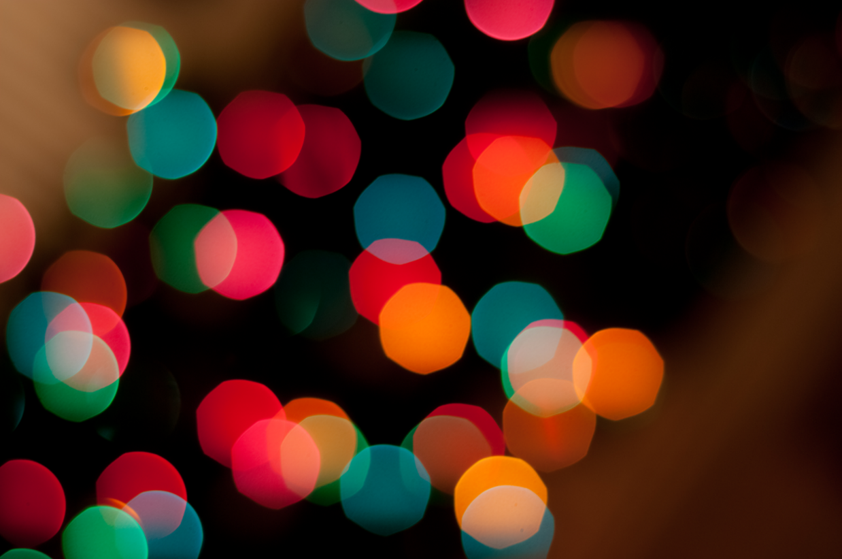
\includegraphics[scale=.75]{Figures/BokehIllustration}
		\caption{Illustration de bokeh}
		\label{fig:bokeh_illustration}
	\end{figure}
	
	\par Une deuxième approche, moins évidente au premier abord, est décrite chez Hoorn \citep{hoorn_virtual_2003}: un environnement virtuel sera jugé assez réaliste s'il remplit sa fonction ; si, dans le cadre d'une application d'apprentissage par exemple, ce qui doit être appris est appris, et si cet apprentissage en RV est transféré en-dehors du monde immersif. Cette définition se détache complètement d'une volonté d'un réalisme d'apparence (comme on a pu voir précédemment) et peut même se détacher d'une construction logique et/ou anthropomorphe de l'environnement virtuel. Si une scène faite de volumes géométriques colorés flottants dans un espace monochrome suffit à transmettre le message voulu, la scène est jugée réaliste.
	
	\par On trouve, dans \citep{fuchs_traite_2003}, une définition plus complète, divisée en cinq acceptations du terme \textit{réalisme} dans le domaine de la RV. Ces acceptations ne sont pas mutuellement exclusives mais il peut être nécessaire d'utiliser plusieurs d'entre elles pour construire sa définition du réalisme:
	\begin{itemize}
		\item Évaluation subjective du degré de ressemblance d'une situation.
		\item Fidélité de construction de la simulation aux lois de la Nature.
		\item Évaluation subjective du degré de crédibilité d'une situation.
		\item Fidélité psychologique.
		\item Illusion du réel (connue aussi sous l'appellation \textit{présence}).
	\end{itemize}
	
	\par La première acceptation, l'évaluation subjective du degré de ressemblance, a déjà été décrite dans un paragraphe précédent. Elle recouvre toute la partie esthétique et artistique de la conception de l'environnement virtuel.
	
	\par La deuxième acceptation, la fidélité de la simulation aux lois de la Nature, accorde moins d'importance à la beauté de la simulation qu'à son comportement simulé ; en dépit de ce que peut juger l'utilisateur. Chaque fonctionnalité implémentée se comporte en suivant un modèle issu du monde physique réel. De par le biais de perception qui peut être induit dans un monde virtuel, les comportements (comme par exemple la gravité, l'adhérence sur un sol, etc ...) et/ou les apparences (rendu des couleurs, floutage des images en fonction de la vitesse, ...) peuvent apparaitre comme non naturels à l'utilisateur. Son avis n'est pas pris en compte, on se contente d'afficher des modèles rigoureux.
	
	\par La troisième acceptation, est la création d'une expérience perceptive qui serait crédible du point de vue du système sensoriel, tant sur le plan microscopique (chaque élément pris à part) que sur le plan macroscopique (l'environnement virtuel dans sa globalité). Même si les informations qui sont envoyées à l'utilisateur (via l'interface de l'environnement virtuel) ne suivent pas rigoureusement les lois de la physique et du monde \textit{réel}, il faut que l'observateur les perçoive comme étant vraies.
	
	\par On peut supposer un lien fort et systématique entre cette dernière acceptation (perception crédible) et la précédente (construction objective via des modèles déterminés) mais cette question est encore grande ouverte et sujette à recherche.
	
	\par Ensuite, la quatrième acceptation du terme \textit{réalisme} est liée à une fidélité d'ordre psychologique. L'utilisateur doit se comporter de la même manière dans l'environnement virtuel que dans la même situation dans le monde physique. Les images affichées peuvent ne pas correspondre avec ce que l'utilisateur verrait dans la situation réelle (en fonction de la tâche à réaliser) tant que les performances et les résultats du sujet dans l'environnement virtuel sont similaires ou identiques à celles/ceux enregistré(e)s dans le monde réel. Cette acceptation est largement détaillée dans la littérature \citep{patrick_training:_1992,stoffregen_one_2003,burkhardt_realite_2003}.
	
	\par Enfin, la cinquième et dernière acceptation fusionne les concepts de \textit{réalisme} et de \textit{présence}. Plus le sentiment de présence dans un environnement virtuel sera fort, plus le réalisme dudit environnement le sera aussi. La présence est <<~l'illusion d'une réalité qui n'existe pas~>> \citep{stoffregen_one_2003}, c'est à dire le fait de faire croire au cerveau que les images/objets/personnes virtuelles que l'on voit sont en fait bien réels ou vivants \citep{burkhardt_realite_2003}. Plus la croyance en la réalité de la scène est forte, plus la présence est forte.
	
	\begin{figure}[h]
		\centering
		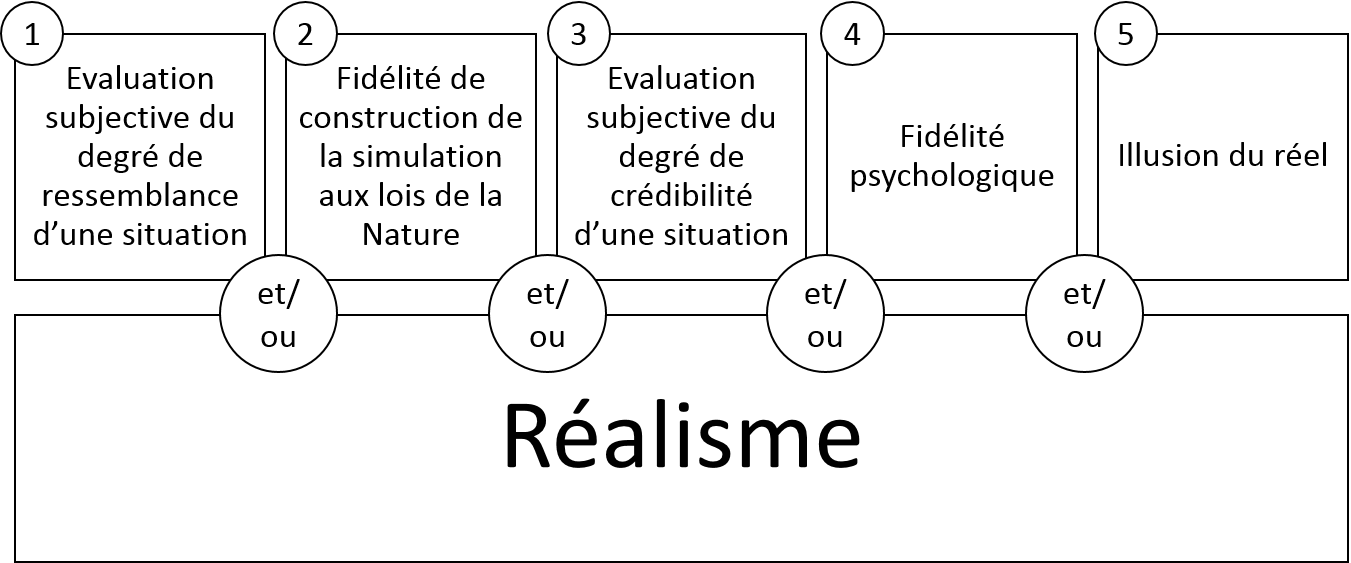
\includegraphics[scale=.65]{Figures/AcceptationsRealisme}
		\caption{Différentes acceptations du terme \textit{réalisme} chez \cite{fuchs_traite_2003}}
		\label{fig:acceptations_realisme}
	\end{figure}
	
	\section{Définition de la multi-sensorialité 3D}
	\subsection{Immersion}
	\par Deux sémantiques coexistent: l'immersion est à la fois l'action d'immerger un utilisateur dans un environnement complètement virtuel via des images de synthèse ; mais c'est aussi l'effet (avéré ou non) qu'a cette immersion sur ce même utilisateur. De manière plus formelle, on peut dire que l'immersion est le <<~degré et [la] qualité, par l'interface [d'un] système, du contrôle des entrées sensorielles pour chaque modalité de perception et d'action~>> (depuis \citep{fuchs_traite_2003}).
	
	\par Pour \cite{burkhardt_conception_1999}, le degré d'immersion est caractérisé par un ensemble de grandeurs:
	\begin{itemize}
		\item Le sous ensemble des modalités mises en œuvre dans l'interaction.
		\item Les propriétés des dispositifs d'interaction pour chacune des modalités visées (degré de complétude, qualité, paramètres du signal, ...)
		\item La cohérence interne et la latence globale de l'information et des réactions délivrées en temps réel par le système.
		\item Les propriétés physiques de l'environnement physique dans lequel se déroule l'expérience.
	\end{itemize}
	
	\subsection{Présence}
	\par Le concept de présence rassemble à la fois le(s) résultat(s) et l'effet d'une (bonne) immersion. Comme décrit dans \citep{burkhardt_realite_2003}: <<~[la présence] désigne l'effet de faire percevoir comme réels ou vivants, les objets, évènements ou personnages avec lequel l'utilisateur interagit dans l'environnement virtuel~>>.
	
	\section{Cadre d'étude}
	\par Dans notre cas, la définition du réalisme qui aura été retenue -et qui sera sous-entendue quand on utilisera le mot \textit{réalisme} seul- est celle de la proximité physiologique avec le système visuel humain.
	
	\par Le but de cette thèse n'est pas de construire de nouveaux modèles esthétiques et de travailler à l'amélioration graphique des simulateurs (objectif qui incombe plutôt à un designer ou à un graphiste), ni d'élaborer un nouveau modèle de vision mais plutôt de travailler avec des modèles de vision, c'est à dire la manière dont la caméra virtuelle va extraire les informations de la scène virtuelle -par opposition aux modèles d'affichage qui décrivent comment les informations capturées par la caméras doivent être affichées sur le(s) écran(s)- pour déterminer des caractéristiques qui soient proches des facultés de la vision humaine.
	
	\begin{figure}[h]
		\centering
		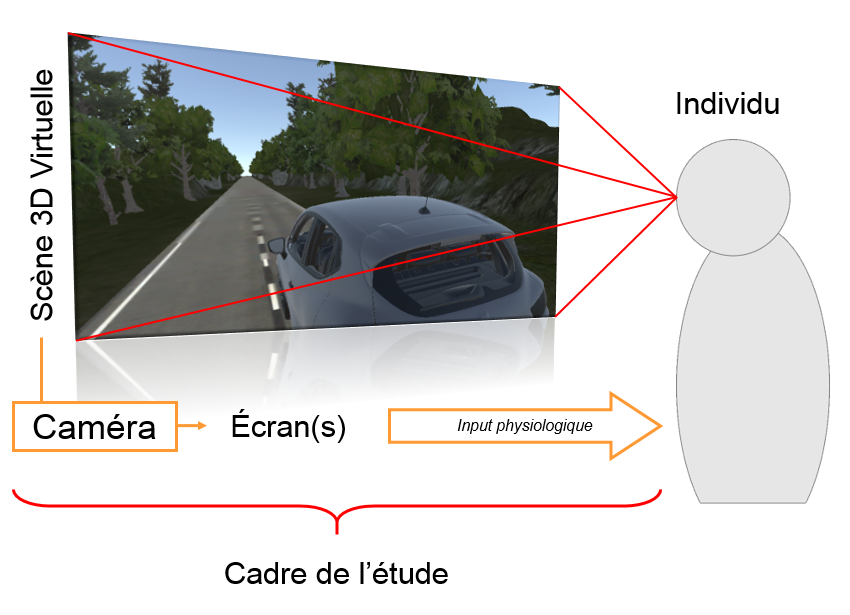
\includegraphics[scale=.65]{Figures/CadreEtude}
		\caption{Cadre d'étude de la thèse}
		\label{fig:champ_d_etude_these}
	\end{figure}
	
	\par Nos travaux dépassent le simple cadre du réalisme en tant que tel, de par leur implication dans le domaine de la Réalité Virtuelle: par construction, celle-ci met en jeu tous les sens de l'homme. \citep{burdea_realite_1993} résument bien en disant que <<~de part sa nature même, c'est à dire de par ses caractéristiques d'immersion et d'interactivité, le système de RV implique "presque tout l'homme": tous ses sens, toute son attention~>>.
	
	\par Dans le cadre de la thèse, le sens de <<~multi-sensorialité~>> n'est donc pas l'usage de plusieurs des cinq sens traditionnels (ouïe, vue, odorat, toucher et goût) mais plutôt la prise en compte de la temporalité de l'expérience et de la capacité de l'observateur à bouger dans son environnement, au bénéfice de la vision. Par exemple, la parallaxe de mouvement est mécaniquement réalisée par le mouvement de la tête et apporte des informations de profondeur pour la vision. Cela nous permettra d'englober les concepts de présence et d'immersion dans la réflexion autour de la thèse, avec ses impératifs de cohérence et de qualité de l'expérience utilisateur que cela implique.
	
	\par Le réalisme physiologique doit, par construction et par définition, se baser sur le système visuel humain. Dans la suite de ce chapitre, nous passerons en revue un grand nombre de paradigmes de la vision afin d'établir précisément la compréhension de son fonctionnement.

\chapter{Fonctionnement général de la vision}
\par Première interface et premier organe de la chaine, l'œil -à contrario de ce qui est généralement pensé- n'est pas la pièce maitresse de la vision: il ne sert \textit{qu'à} envoyer des signaux électriques au cerveau et pourrait être remplacé par une caméra par exemple, dans la mesure où celle-ci émet les bonnes informations à travers le nerf optique \citep{dobelle_artificial_2000}. L'œil reste néanmoins un outil très puissant et versatile. Nous allons ici rappeler le fonctionnement de l'œil et de la vision, qui se traduit par les informations collectées et transmises par l'œil puis traitées par le cerveau. Le sujet est tout à fait connu et largement documenté \citep{fairchild_human_2005,wandell_foundations_1995,gross_human_2008,driscoll_eyes_1978}.

	\section{Structure de l'œil}
	\par L'œil se divise en un certain nombre de parties dont les principales sont la cornée, l'iris, la pupille, le cristallin, la rétine et les deux chambres contenant les humeurs aqueuse et vitrée. Toute la structure de l'œil est résumée sur la Fig. \ref{fig:oeil}.
	
	\par La cornée est la première interface entre l'extérieur et l'intérieur de l'œil.
	
	\par Le cristallin est la lentille principale de l'œil et va s'occuper de la netteté du monde qui nous entoure via le processus d'accommodation. Le principe est simple: il faut placer le foyer image de l'œil sur la rétine (voir Section suivante). Pour ce faire, l'œil accommode, c'est à dire qu'il va modifier sa géométrie dans le but de modifier ses propriétés optiques. Dans la pratique, les muscles ciliaires font se déformer le cristallin (voir Fig. \ref{fig:oeil}) en réduisant sa hauteur et donc en augmentant sa convexité ou inversement. Ce processus dure 1 seconde et n'est pas définitif: une fois l'œil accommodé, celui-ci oscille légèrement autour de la valeur  d'accommodation, à une fréquence de 5 Hz. Ce mécanisme permet de récupérer des retours d'information en cas d'ajustements à opérer \citep{gross_human_2008}.
	
	\par Le mécanisme d'accommodation ne fonctionne plus à partir d'un certain seuil de luminosité. Ce seuil est évalué à $0.01~cd/m^2$. En l'absence d'accommodation, l'œil prend une position intermédiaire entre la position relâchée (accommodation à l'infini) et une position \textit{presque-accommodée} \citep{gross_human_2008}.
	
	\par Ensuite, la pupille et l'iris sont intimement liées car la première est l'espace laissé par la seconde au centre de l'œil. L'iris est une composante contrôlable de l'œil. L'iris contrôle la quantité de lumière qui arrive dans l'œil et donc sur la rétine. Plus la pupille sera grande, plus la lumière pourra rentrer dans l'œil. Un œil humain peut supporter des luminosités (luminances) allant de $10^{-6}$ à $10^5~cd/m^2$. La variation du diamètre de la pupille peut être modélisée par un modèle mathématique. S'il en existe un certain nombre dans la littérature (voir \citep{watson_unified_2012} pour un état de l'Art exhaustif), on donne ici l'équation suivante (Eq. \ref{eq:diam_pupille}). De la même manière que l'accommodation, le diamètre de la pupille oscille autour de sa valeur moyenne à l'instant t. Ce phénomène est appelé \textit{hippus} \citep{gross_human_2008}.
	
	\begin{equation}
		log_{10}(D_{iris}) = 0.8558 - 0.000401 \cdot [8.1 + log_{10}(L)]^3
		\label{eq:diam_pupille}
	\end{equation}
	
	\par De la même manière, la vergence est la capacité des yeux de s'orienter vers le point d'accommodation lorsque celui est proche. On appelle convergence le phénomène qui consiste à augmenter l'angle formé par l'intersection des lignes du regard de chaque œil (quand la cible se rapproche) et divergence le cas inverse, lorsque cet angle diminue (la cible s'éloigne). Le processus possède une latence estimée à 150 ms et une durée approximative évaluée à 0.2 - 0.6 secondes \citep{devisme_optimisation_2004, gross_human_2008}.
	
	\par L'œil humain a une taille globalement constante entre les individus: autour de 24 mm de diamètre \citep{glassner_principles_1995}. Le pouvoir optique de l'œil, c'est à dire sa capacité à adapter ses propriétés optiques, se mesure en dioptries. Les dioptries ($\delta$) sont l'inverse de la distance focale d'un système optique, elles sont homogènes à des $m^{-1}$. Faire varier ses dioptries (et donc sa distance focale) permet l'accommodation et l'adaptation de l'œil. L'œil humain demande environ 42$\delta$ en fonctionnement et peut monter jusqu'à une puissance nécessaire de 60 à 80$\delta$ pour compenser les défauts de l'œil \citep{glassner_principles_1995}, au nominal.
	
	\par La rétine tapisse le fond de l'œil et est composée de millions de récepteurs photosensibles qui vont être responsables de la captation de l'image. Ces photo-récepteurs sont les cônes, sensibles à la couleur, et les bâtonnets sensibles à la luminosité. Il existe 3 types de cônes, qui sont chacun sensibles à différentes longueurs d'onde: on retrouve les cônes de type S (pour \textit{small}, petite longueur d'onde) avec un maximum de sensibilité à $420~nm$ ; ensuite, on trouve les cônes de type M (pour \textit{medium}, moyenne longueur d'onde) avec un maximum de sensibilité à $530~nm$ ; et enfin, on a les cônes de type L (pour \textit{long}, grande longueur d'onde) avec un maximum de sensibilité à $560~nm$. Le seul message émanant d'un cône ou d'un bâtonnet est celui de son activation. La reconnaissance des couleurs et de l'intensité de la lumière se fait par la combinaison des résultats d'activation des différents types de cônes ; ce procédé est analogue à celui du tramage\footnote{Tramage: Procédé permettant de générer de nouvelles couleurs à partir d'une base limitée de couleurs. Typiquement, en informatique, les pixels des écrans sont en fait composés de 3 sous pixels: blanc, rouge et vert. Une fois combinés et vus d'assez loin, ils semblent ne créer qu'une seule couleur, potentiellement différente.} en informatique. Alors que l'on pourrait penser qu'il existe un cône dédié à chaque couleur, l'œil humain ne possède que trois types de cônes. En effet, si l'œil possédait de nombreux autres types de cône, la densité par cône serait grandement réduite et donc la finesse de vision avec \citep{glassner_principles_1995}.
	
	\par Les cônes et les bâtonnets ont chacun leur plage de fonctionnement optimale. Dans le domaine photopique (lumière du jour), les bâtonnets sont saturés en luminosité et sont beaucoup moins efficaces que dans le domaine scotopique (de nuit). De leur côté, les cônes adaptent leur maximum de saturation par rapport au niveau global d'illumination \citep{glassner_principles_1995}.
	
	\par La répartition des cônes et des bâtonnets sur la rétine n'est pas du tout homogène (voir Fig. \ref{fig:densite_cones_batonnets}). Une zone de la rétine présente une extrême concentration de cônes. Cette zone est appelée \textit{fovéa}. De par l'utilité des cônes et par construction du système optique de l'œil, c'est l'endroit où les rayons lumineux issus de la cible regardée convergent. On retrouve, en périphérie de la fovéa, les bâtonnets. Ce qui est capté par la fovéa est vu net, tandis que ce qui est capté par les bâtonnets ne l'est pas. L'axe de vision est d'ailleurs défini par le rayon issu du point nodal image jusqu'à la fovéa (voir section suivante). Cet axe, représenté sur la Fig. \ref{fig:modele_liou_brennan} est donc fixe et l'angle qu'il forme avec l'axe optique de l'œil (ici appelé \textit{alpha}) vaut entre 3 et 8 degrés suivant les individus \citep{gross_human_2008}.
	
	\par La rétine n'est que la première étape du système d'acquisition et la totalité de celui-ci ainsi que le traitement par le cerveau sera traité plus loin dans le chapitre. D'abord, nous nous concentrons sur la modélisation de l'œil.
	
	\begin{figure}[h]
		\centering
		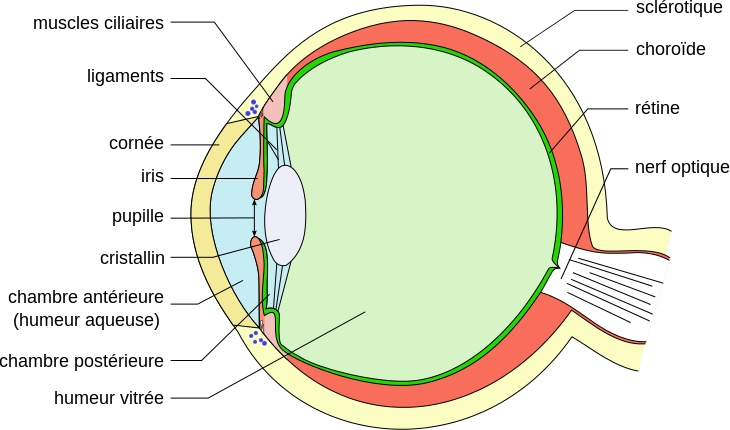
\includegraphics[scale=.4]{Figures/SchemaOeil}
		\caption{Structure de l'œil}
		\label{fig:oeil}
	\end{figure}
	
	\begin{figure}[h]
		\centering
		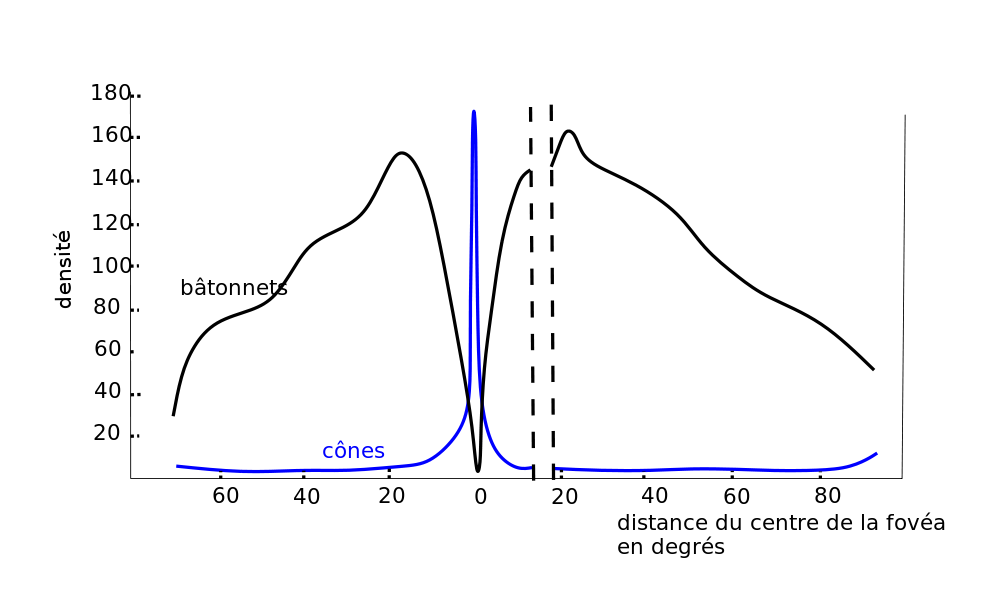
\includegraphics[scale=.5]{Figures/DensiteConesBatonnets}
		\caption{Répartition (en $milliers/mm^2$) des cônes/bâtonnets sur la rétine}
		\label{fig:densite_cones_batonnets}
	\end{figure}
	
	\section{Modélisation de l'œil}
	\par De nombreux scientifiques se sont intéressés à la compréhension et la modélisation de l'œil, et ce, dès la moitié du XIXe siècle avec Carl Friedrich Gauss qui en a défini les grands principes optiques. Cependant, avant de discuter des différents modèles de l'œil qui ont pu émerger au cours (notamment) du XXème siècle, il parait nécessaire de re-poser certaines bases élémentaires de l'optique géométrique.
	
	\par On note quelques points particuliers dans un système optique simple (type lentille concave ou convexe). De manière générale, on rappelle que les points caractéristiques d'un lentille sont qualifiés d' \textit{objet} quand ils sont avant la lentille (en terme de trajet du rayon lumineux) et d' \textit{image} lorsqu'ils sont après la lentille. Par convention, un point caractéristique est noté avec une lettre majuscule tandis que son point conjugué image est noté avec la même lettre agrémentée d'un \textit{prime}.
	\begin{itemize}
		\item Le foyer objet est le point à partir duquel les rayons émergents sont ensuite dirigés vers l'infini optique (c'est à dire parallèle à l'axe optique) après passage par la lentille. Le foyer objet est noté F.
		\item Le foyer image est le point vers lequel convergent tous les rayons issus de l'infini avant la lentille. Dans le cas d'un œil sain (sans problèmes ophtalmologiques de type myopie ou hypermétropie), ce point doit être confondu avec la rétine pour avoir une image nette. Comme on a pu voir précédemment, c'est là le principal mécanisme de l'accommodation qui va déformer le système optique pour déplacer les foyers afin de faire la netteté sur la rétine. Le foyer image est noté F'.
		\item Le point central, par lequel un rayon passe sans être dévié (qui correspond au centre de rotation de l'œil). Il est noté C.
		\item Le point nodal objet est un point très particulier parce qu'il peut être considéré comme l'équivalent du \textit{point de vision}, c'est à dire le point où on pourrait ramener l'intégralité de l'œil à un équivalent ponctuel. Dans un système optique, il est défini comme le point par lequel passe un rayon lumineux avec une incidence donnée et ressort au point conjugué avec la même incidence. Il n'existe que dans un système optique complexe (fait de plusieurs lentilles ou interfaces optiques). Dans le cas d'une lentille simple seule il est confondu avec le centre. Ce point est globalement situé 6 mm à l'avant du centre de l'œil, sur l'axe optique \citep{gross_human_2008,ogle_optics:_1968}. Les points nodaux sont notés N et N'.
	\end{itemize}
	
	\begin{figure}[h]
		\centering
		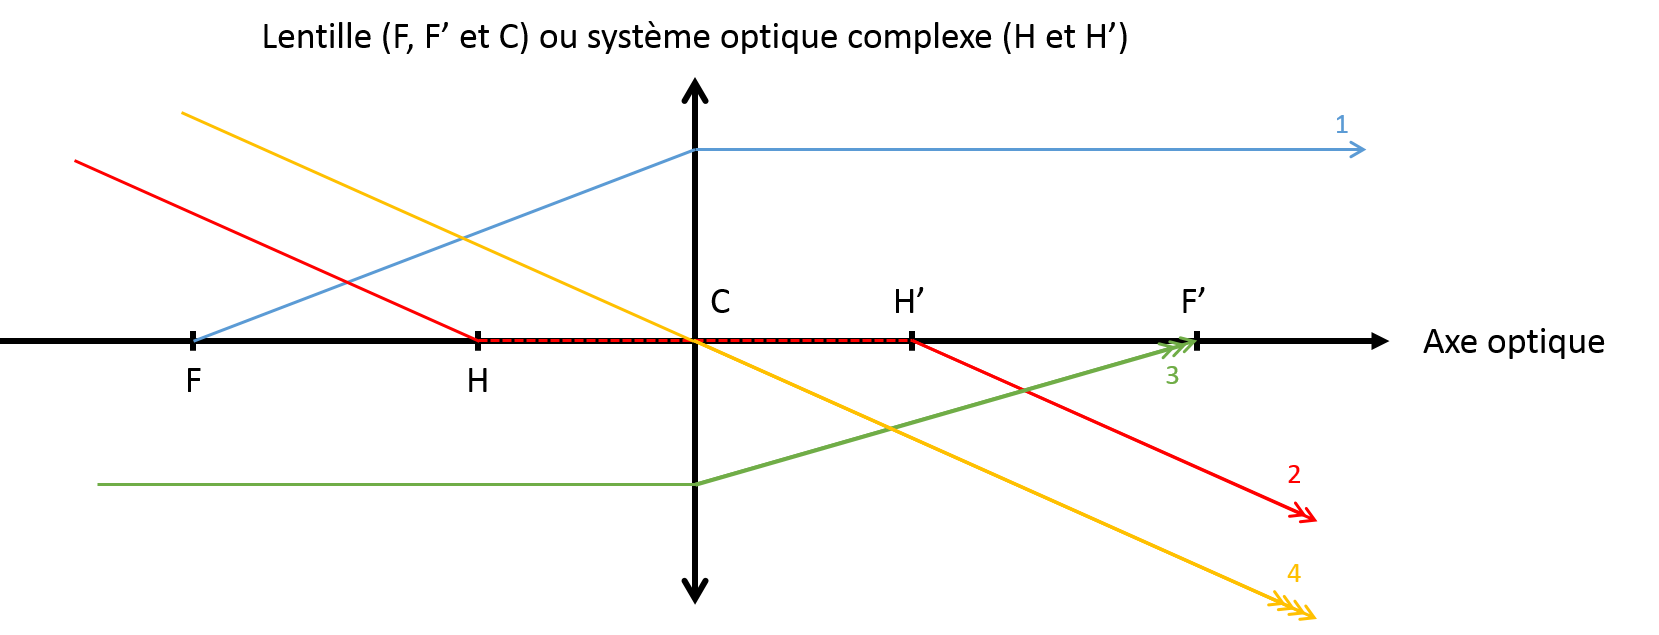
\includegraphics[scale=.5]{Figures/PointsSystemeOptique}
		\caption{Points caractéristiques (cardinaux) d'un système optique plan}
		\label{fig:points_cardinaux_systeme_optique}
	\end{figure}
	
	\par L'œil possède deux axes principaux: l'axe optique, qui passe par les centres de toutes les surfaces optiques ou composantes de l'œil (cristallin, pupille, ...) et l'axe de vision qui est composé en fait de deux demi-axes que sont les rayons qui passent par les points nodaux et jusqu'à la fovéa. L'œil est orienté selon l'axe optique mais la vision se fait le long de l'axe dit \textit{de vision}. La vision hors axe est appelée \textit{vision périphérique}.
	
	\par Enfin, un grand nombre de modèles de l'œil ont été proposés, plus ou moins complexes, avec notamment des variations sur le nombre de surfaces optiques, jusqu'à l'adoption du modèle de \citep{liou_anatomically_1997}. Malgré tout, ce modèle est tout sauf définitif et est toujours susceptible d'être amélioré ou affiné dans le futur. On présente une liste non-exhaustive des différents modèles de l'œil qui ont pu être élaborés au cours du XXème siècle \citep{liou_anatomically_1997,gross_human_2008}:
	\begin{itemize}
		\item Modèle de Helmholtz - Laurence (1909)
		\item Modèle de Gullstrand (1911): modèle le plus utilisé, notamment car un grand nombre de distances (taille de l'œil, distances focales, distance de la pupille, ...) et tous les indices de réfractions des différents milieux de l'œil y sont reportés (voir Fig. \ref{fig:modele_gullstrand}). Le modèle optique théorique pour la propagation de la lumière est composé de 3 surfaces.
		\item Modèle de Emsley (1946): modèle simplifié réduit à 1 seule surface.
		\item Modèle de Lotmar (1971): modélisation de la cornée et de la face arrière du cristallin par des surfaces polynomiales (plutôt que des sections de sphère).
		\item Modèle de Kooijman (1983): modèle en 4 surfaces, ajout d'asphéricités sur les surfaces sphériques.
		\item Modèle de Navarro (1985): idem que Kooijman avec des effets chromatiques additionnels, tels que la dispersion de la lumière.
		\item Modèle de Schwiegerling (1995)
		\item Modèle de Liou \& Brennan (1997): modèle à 5 surfaces dont 1 purement théorique (voir Fig. \ref{fig:modele_liou_brennan}). C'est la modèle le plus utilisé dans le domaine du calcul et de la simulation de rayons. 
	\end{itemize}
	
	\begin{figure}[h]
		\centering
		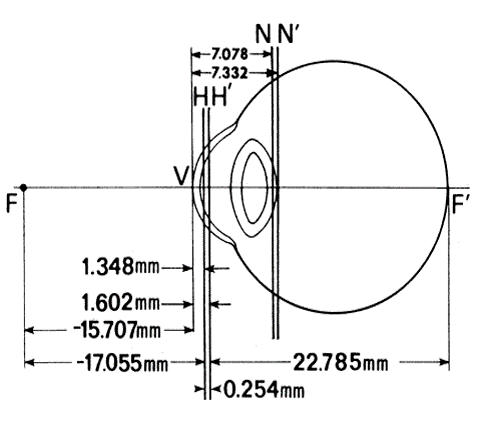
\includegraphics[scale=1.25]{Figures/GullstrandModel}
		\caption{Modèle et valeurs physiologiques de Gullstrand}{Image tirée de \citep{liou_anatomically_1997}}
		\label{fig:modele_gullstrand}
	\end{figure}
	
	\begin{figure}[h]
		\centering
		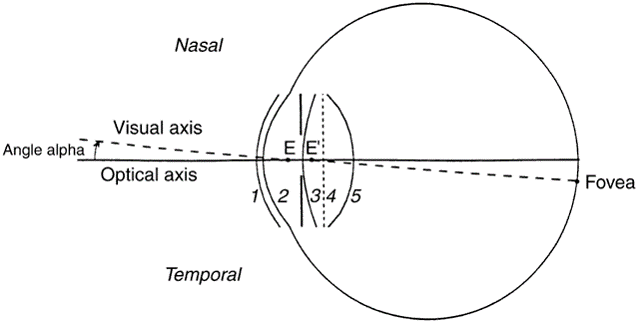
\includegraphics[scale=1]{Figures/LiouBrennanModel}
		\caption{Modèle de Liou \& Brennan}{Image tirée de \citep{liou_anatomically_1997}}
		\label{fig:modele_liou_brennan}
	\end{figure}
	
	\par Jusqu'à présent, nous avons détaillé le fonctionnement d'un œil seul. Nous allons maintenant nous intéresser à la vision binoculaire, c'est à dire de deux yeux en même temps.
	
	\section{Vision binoculaire}
	\par La vision binoculaire est avant tout un excellent outil de compréhension de l'environnement qui nous entoure, et notamment de la profondeur: le cerveau peut comparer en temps réel deux points de vue légèrement différents et en tirer des conclusions.
	
	\par Les disparités sont les éléments nécessaires au fonctionnement de la vision binoculaire. Ce sont les différences de position relative entre les deux images perçues (une par œil) d'un même objet. Si un objet est pleinement centré sur l'image perçue par l'œil gauche, il sera vu légèrement décalé du centre par l'œil droit.	Il existe deux types de disparités; les disparités verticales et les disparités horizontales \citep{devisme_optimisation_2004}.
	
	\par Les disparités horizontales sont générées par une différence angulaire sur le plan de l'azimut. Elles sont en charge de la perception relative de la distance, c'est à dire à la perception de la profondeur (relief).
	
	\par Les disparités verticales sont issues de la perception par les yeux d' une différence d'élévation pour le même point. Elles peuvent aussi apparaitre si un des yeux est plus proche de l'objet que l'autre (on parle alors de grossissement différentiel). Les disparités verticales permettent d'estimer la distance absolue d'un objet ainsi que l'excentricité d'une surface, indépendamment de son orientation.
	
	\par En imagerie 3D, et plus spécifiquement en Réalité Virtuelle, les disparités peuvent être source de fatigues dans le système visuel humain. Ce problème a été adressé notamment en ajoutant du flou sur les disparités les plus grandes, en ajoutant un flou périphérique pour reproduire le flou rétinien et en proposant un modèle de caméras convergentes qui génère des disparités plus conformes à la réalité \citep{aurat_immersion_2016}.
	
	\par L' horoptère est le lieu des points de disparité horizontale nulle pour un point de fixation donné, c'est à dire, à un instant t donné, lorsqu'on regarde à un endroit donné, il existe une infinité de points pour lesquels aucun disparité n'est perçue: ils sont au même endroit sur l'image perçue par l'œil gauche et par celle perçue par l'œil droit. Théoriquement, le lieu de ces points est un cercle passant par le point de fixation et par le premier point nodal (point nodal objet, H) de chaque oeil; ce cercle s'appelle le Cercle de Vieth-Müller. Dans la pratique, le lieu de l'horoptère n'est pas tout à fait un cercle et présente une légère déviation, nommée Déviation de Hering-Hillebrand (voir Fig. \ref{fig:horoptere_panum}) \citep{neveu_impact_2012}.
	
	\par Si on prend en compte les disparités verticales, le lieu des points de disparité horizontale-verticale nulle devient un cylindre (Extension du Cercle de Vieth-Müller).
	
	\begin{figure}[h]
		\centering
		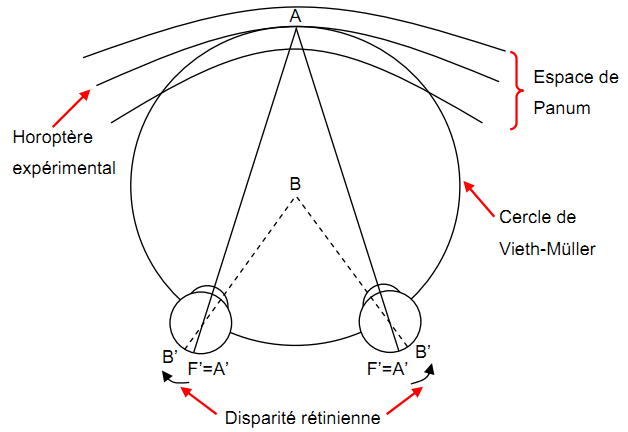
\includegraphics[scale=.55]{Figures/HoropterePanum}
		\caption{Horoptères théorique et empirique, Aire de Panum et disparités rétiniennes.}{Image tirée de \citep{neveu_impact_2012}.}
		\label{fig:horoptere_panum}
	\end{figure}
	
	\par L'œil possède une certaine capacité à adapter sa puissance (comme vu précédemment). On retrouve cette capacité au niveau du cerveau pour la fusion stéréoscopique. Dans une zone proche autour de l'horoptère (Aire de Panum) le cerveau écrase les disparités et fusionne quand même les images perçues par les yeux. L'étendue et la forme de l'aire de Panum est grandement dépendante des caractéristiques locales du stimulus \citep{devisme_optimisation_2004}.
	
	\par Enfin, la vision binoculaire est tributaire d'une certaine acuité stéréoscopique, c'est à dire la capacité à percevoir un écart de profondeur entre deux plans à une distance donnée. Celle ci est présentée et son modèle démontré à plusieurs endroits \citep{fuchs_traite_2003, gross_human_2008} et sera abordée dans un chapitre suivant. Toutefois, si l'âge et le niveau d'accommodation n'ont pas l'air d'affecter l'acuité stéréoscopique, cette dernière est dépendante du contraste et de la quantité d'éclairement rétinien \citep{devisme_optimisation_2004}.
	
	\section{Traitement post-rétinien}
	\par Nous allons maintenant aborder toute la partie transmission et traitement par le cerveau du signal émis par les rétines. Le comportement précis dans le cerveau est encore à ce jour une question ouverte que nous traiterons donc dans les limites du possible et de l'utile dans le cadre de cette thèse. On se base notamment sur \textit{Neurosciences: A la découverte du Cerveau} de \citep{bear_neurosciences:_2007}, ouvrage particulièrement instructif.
	
	\par Tout d'abord, il convient de développer quant à la structure même des cônes, de quelle manière ceux-ci jouent leur rôle de transducteur\footnote{Transducteur: Dispositif assurant une conversion ou un transfert de signaux et dans lequel un signal au moins est de nature électrique. (s.d.). Dans \textit{Dictionnaire Larousse en ligne}. Repéré à \url{http://www.larousse.fr/dictionnaires/francais/transducteur/79088}}: transformant un signal lumineux entrant en signal électrique sortant.
	
	\par La rétine est en fait composée de plusieurs types de cellules intermédiaires, les cônes et les bâtonnets n'étant qu'en bout de chaîne: cellules ganglionnaires, cellules amacrines, cellules horizontales et cellules bipolaires (voir Fig. \ref{fig:structure_retine}) \citep{bear_neurosciences:_2007}. Ces cellules se réunissent ensuite pour former le nerf optique et sortir de l'œil. Parmi les cellules ganglionnaires il en existe plusieurs types, chaque type véhiculant des informations différentes \citep{anses_effets_2014}.
	
	\par La voie magnocellulaire (M) représente 5\% de la population de cellules ganglionnaires. Ces cellules sont sensibles aux contrastes de luminance et ont une vitesse de conduction plutôt rapide. Elles sont à relier à la voie dorsale (voir plus loin).
	
	\par La voie parvocellulaire (P) représente 90\% de la population de cellules ganglionnaires. Ces cellules sont sensibles aux couleurs et, malgré une vitesse de conduction plus lente que les cellules de la voie M, elles répondent de manière tonique aux stimulations. Ces cellules sont à rapprocher de la voie ventrale.
	
	\par Enfin, il existe une voie non M - non P qui représente les 5\% de population restants et participe à d'autres tâches que la vision pure (voir plus loin). 
	
	\begin{figure}[h]
		\centering
		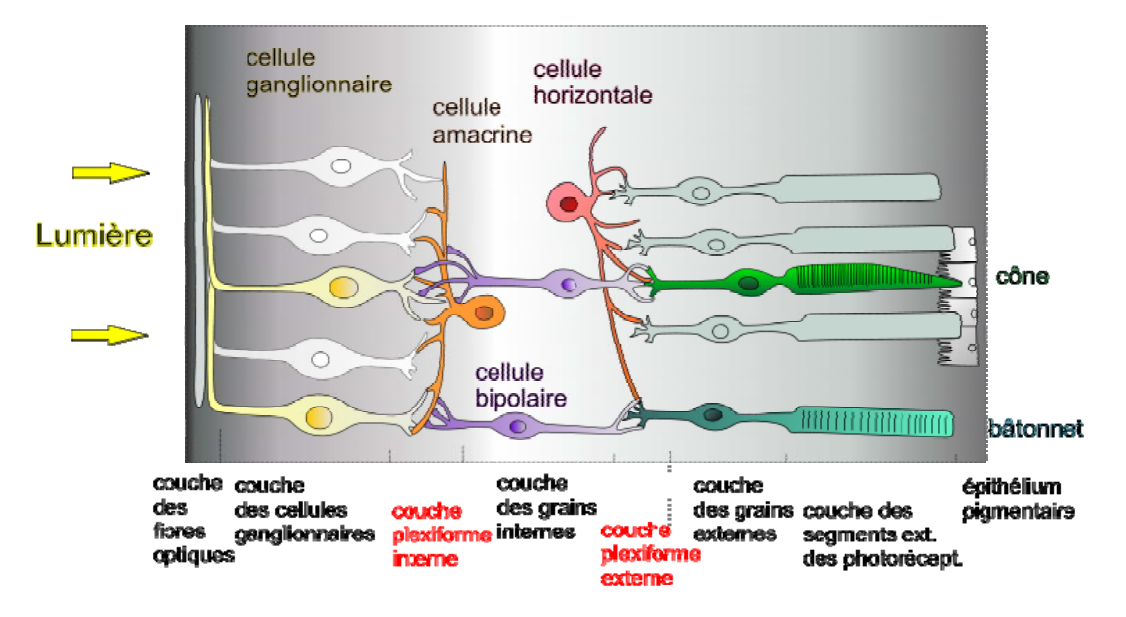
\includegraphics[scale=.45]{Figures/StructureRetinae}
		\caption{Structure et cellules composant la rétine}{Image tirée de  \citep{anses_effets_2014}.}
		\label{fig:structure_retine}
	\end{figure}
	
	\par Une fois le signal lumineux transformé dans une des trois voies (M, P ou non M - non P), l'information circule dans le nerf optique en direction du cerveau. Les nerfs optiques de chaque œil se croisent au niveau du chiasma optique avant de continuer leur chemin dans le tractus optique et d'arriver au cerveau. Au niveau du chiasma, les fibres porteuses des informations visuelles sont redirigées: les fibres des deux moitiés gauches des yeux sont envoyées à la partie droite du cerveau, tandis que les fibres des deux moitiés droites des yeux sont envoyées à la partie gauche.
	
	\par L'interface entre le cerveau à proprement parler et le tractus optique s'appelle le CGL (Corps Genouillé Latéral). Le CGL est composé de 6 couches qui vont permettre la distribution de l'information dans les différents cortex visuels. Les informations issues de la voie M sont attribuées aux couches 1 et 2 du CGL, tandis que les informations de la voie P sont attribuées aux couches 3, 4, 5 et 6 du CGL. Les 5\% d'informations restantes (la voie M non P) ne va pas dans le CGL (et donc dans les cortex d'analyse de l'image) mais se dirige dans la mésencéphale et l'hypothalamus. Ces deux dernières aires du cerveau sont dédiées à la gestion du reste du corps humain: régulation du bio-rythme, sécrétion des hormones du sommeil, gestion de l'attention, ...
	
	\par La radiation optique permet de faire le lien, via des neurones, entre les 6 couches du CGL et le Cortex Visuel Primaire (V1) qui marque l'entrée dans le cerveau à proprement parler.
	
	\par Le traitement et la compréhension véritable des informations qui ont transité de l'œil jusqu'au CGL se fait dans les cortex visuels. La cartographie et la compréhension du fonctionnement en cortex dans le cerveau fait l'objet de plusieurs théories. Aux côtés des modèles hiérarchique et des agrégats, c'est l'hypothèse des deux voies \citep{ingle_two_1982, mishkin_object_1983, goodale_neurological_1991} qui prédomine. Cette hypothèse est aussi étendue au fonctionnement de l'audition. On la décrit dans le paragraphe suivant.
	
	\par Le traitement de l'image dans les cortex visuels est décomposé en deux voies, à l'image des voies P et M. A l'arrivée dans le Cortex Visuel Primaire (V1), l'information est divisée en deux boucles de traitement indépendantes: la voie dorsale (appelée aussi pariétale) et la voie ventrale (appelée aussi temporale). La voie dorsale correspond au traitement du mouvement et de la position (\guillemotleft~Where~\guillemotright), elle est constituée des cortex V1, V2, V3, V3A, MT et MST avant d'arriver dans le Cortex Pariétal Supérieur. Cette fonction a une vitesse plutôt lente. De l'autre côté, la voie ventrale s'occupe de la gestion des formes et des couleurs (\guillemotleft~What~\guillemotright) et passe par les cortex V1, V2, VP, V4 et V8 avant d'arriver dans le lobe temporal. Cette voie fonctionne à grande vitesse \citep{dhondt_emotion_2011, kaiser_dorsal_2010}.
	
	\begin{figure}[h]
		\centering
		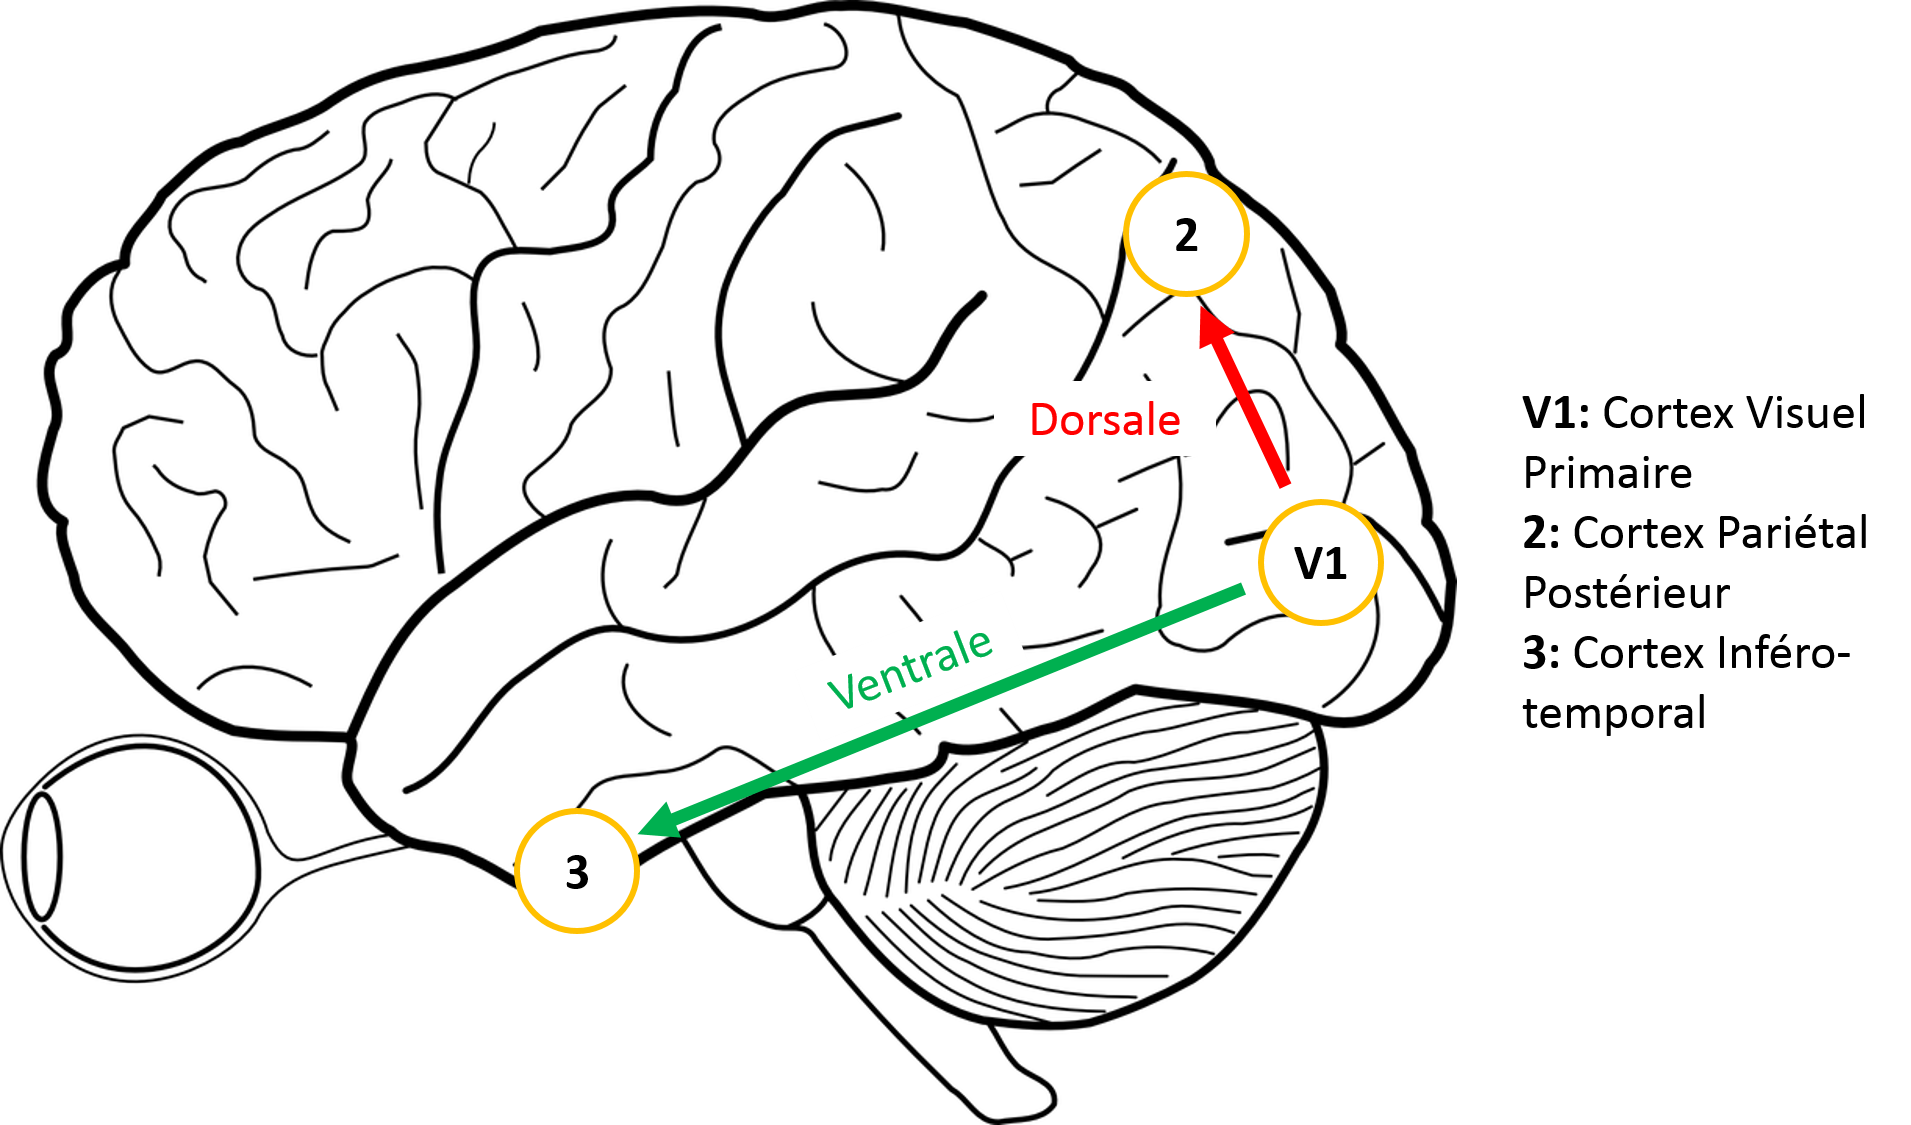
\includegraphics[scale=.35]{Figures/VoiesVentraleDorsale}
		\caption{Direction des voies ventrale et dorsale dans le cerveau.}
		\label{fig:voies_ventrale_dorsale}
	\end{figure}
	
	\par L'information visuelle n'est pas transmise au cerveau telle quelle sous la forme de quatre informations (bâtonnets, cônes S, cônes M, cônes L). Ces signaux de sortie des photo-récepteurs sont additionnés ou soustraits les aux autres pour donner naissance à trois canaux d'information qui eux seront traités par le cerveau. Cette hypothèse de fonctionnement  -la \textit{Théorie des processus antagoniques} proposée pour la première fois par Ewald Hering en 1872- est compatible avec la théorie de la vision trichromatique (\textit{Théorie de Young-Helmholtz}, 1802 puis prouvée en 1861) puisqu'elle intervient immédiatement après dans le traitement de la lumière.
	
	\par Après les photo-récepteurs, le signal lumineux est donc découpé en trois canaux \citep{glassner_principles_1995,winkler_issues_1999}: un canal achromatique (A) et deux canaux chromatiques (R/G pour le canal rouge-vert et B/Y pour le canal bleu-jaune). On retrouvera ces canaux plus tard dans la description des espaces colorimétriques en informatique. Le canal achromatique sert à coder la valeur de luminance et est issu de la somme des signaux émis par les cônes de type M et L, $A \equiv M + L$. Le canal R/G est quant à lui la différence entre les deux précédents canaux M et L ($R/G \equiv M - L$) tandis que le canal B/Y est la différence entre les signaux émis par les cônes de type S et le canal achromatique: $B/Y \equiv S - A$. Ces mécanismes sont résumés dans la Fig. \ref{fig:opponent_colors_theory}.
	
	\begin{figure}[h]
		\centering
		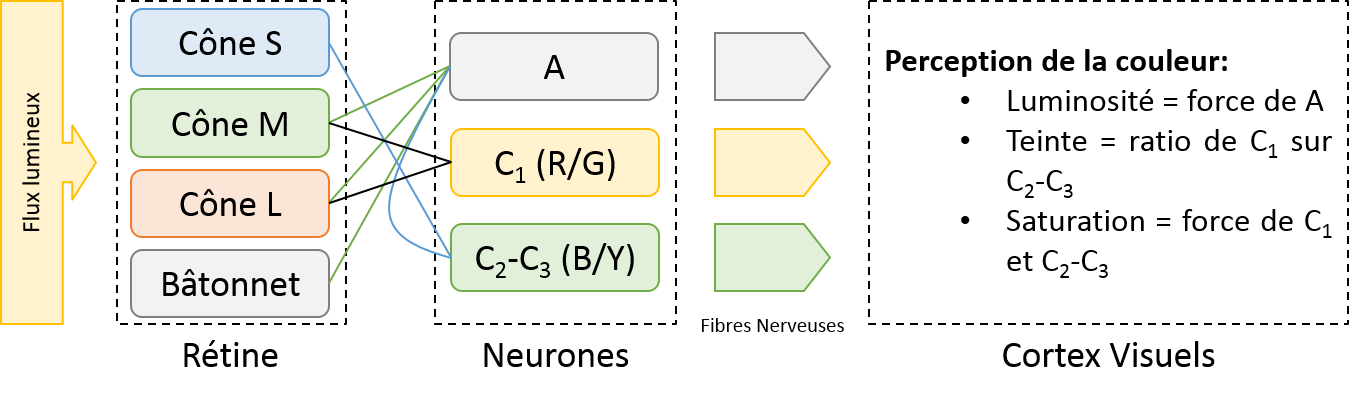
\includegraphics[scale=.6]{Figures/OpponentColorsTheory}
		\caption{Construction des canaux chromatiques et achromatique dans la théorie des processus antagoniques}
		\label{fig:opponent_colors_theory}
	\end{figure}
	
	\par Enfin, le cerveau dénote une certaine sensibilité au contraste (entendu ici comme une variation relative de luminance entre deux points de l'image perçue). Cette sensibilité dépend à la fois de la couleur (on a vu que le canal achromatique était en fait composé des retours de deux types de cônes) et à la fois des fréquences spatiales et temporelles du stimulus lumineux reçu. On peut alors établir des fonctions de sensibilité au contraste (Contrast Sensibility Functions - CSF) \citep{driscoll_eyes_1978,bezzubik_modeling_2015}. La sensibilité au contraste est définie comme l'inverse du seuil de contraste, c'est à dire le minimum nécessaire de contraste suffisant à un observateur pour détecter une variation. On peut trouver des exemples de CSF chez une grand nombre d'auteurs, comme ici avec les CSF moyennes en fonction de la fréquence spatiale du stimulus, pour différentes valeurs d'acuité visuelle (voir Fig. \ref{fig:contrast_sensitivity_functions_acuity}) \citep{owsley_contrast_1983}. On reviendra plus tard, dans une partie spécifiquement consacrée au sujet, sur la perception du contraste.
	
	\begin{figure}[h]
		\centering
		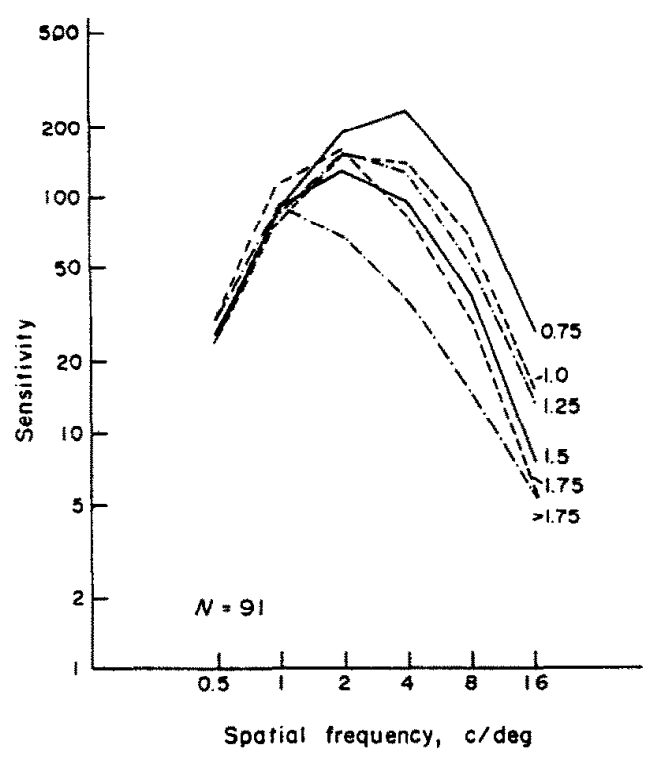
\includegraphics[scale=.45]{Figures/ContrastSensitivityFunctionAcuity}
		\caption{Courbes moyennes de sensibilité au contraste en fonction de la fréquence spatiale du stimulus pour différentes valeurs d'acuité visuelle}{Image tirée de \citep{owsley_contrast_1983}}
		\label{fig:contrast_sensitivity_functions_acuity}
	\end{figure}
	
\chapter{Perception de la couleur}
	\par La perception de la couleur a été théorisée via un certain nombre de concepts, lois ou effets ; on présente ici quelques contributions importantes \citep{le_grand_optique_1972, wyszecki_color_2000,judd_color_1975}. L'organisme régulateur de toutes les connaissances dans le domaine de la couleur est la CIE (ou ICE en anglais): la Commission Internationale sur l'Eclairage. En complément, on développe en annexes les différentes lois et effets qui régissent la perception de la couleur.
	
	\section{Espaces colorimétriques}
	\par Il existe de très nombreux espaces colorimétriques (sRGB, YIQ, YES, YCC, LCh, TekHVC, NCS, Munsell, Coloroid, Pantone, CIECAM97, ... \citep{beretta_understanding_2000}) mais une étude globale poussée sort très largement du cadre de l'étude. Nous nous concentrerons donc à évoquer rapidement les différents espaces principaux adoubés par la CIE.
	
	\par La première modélisation à avoir été déposée par la CIE, en 1931, est l'espace colorimétrique CIE RGB. C'est une première tentative de quantification de la couleur avec des primaires proches des maxima de réponse des cônes. La démarche est donc anthropomorphique et cherche à construire un espace linéaire. L'inconvénient (majeur) de ce système est l'obligation de passer par des composantes négatives pour certaines couleurs très saturées ; on s'éloigne alors du fonctionnement de la vision humaine qui est basée sur l'additivité des couleurs.
	
	\par Les défauts de ce premier espace ont amené la CIE à proposer dans le même temps un autre espace, le CIE XYZ, lui aussi linéaire\footnote{Linéaire: les valeurs des primaires varient linéairement, pas les couleurs perçues: une variation de primaire ne donne pas la même variation de couleur}. Dans ce modèle, Y donne	la luminance tandis que X et Z donnent la chrominance et sont définis positifs par construction.
	
	\par Mais la vision humaine des couleurs n'étant pas linéaire, un nouvel espace est développé par la CIE, en 1960, c'est le CIE UVW. Cet espace est non-linéaire et vise à améliorer l'uniformité de répartition des couleurs\footnote{Uniforme: les couleurs perçues varient de manière linéaire, au contraire de la valeur des primaires dans l'espace colorimétrique}. Dans ce modèle, la composante V correspond en tout point à la composante Y de CIE XYZ (luminance). UVW est supplanté 16 ans plus tard (1976) par CIE U'V'W' dont la variation principale est le changement de la matrice de passage vers XYZ.
	
	\par Enfin, en 1976 également, apparaissent les deux espaces les plus complets et utilisés à l'heure d'aujourd'hui: CIELAB et CIELUV. CIELUV est utilisé pour caractériser les couleurs de lumières tandis que CIELAB sert dans le domaine des couleurs des surfaces. Ils sont basés sur U'V'W' et appartiennent à la famille des espaces uniformes mais non-linéaires. Nous détaillerons ici CIELAB car c'est celui qui est utilisé dans le domaine de l'informatique. Pour de plus amples informations, on conseillera \citep{schanda_colorimetry:_2007}.
	
	\par L'espace CIELAB, de sa vraie dénomination CIE $L^\ast a^\ast b^\ast$, est caractérisé par une composante de clarté $L^\ast$ et deux paramètres $a^\ast~et~b^\ast$ qui expriment l'écart de la couleur par rapport à une surface grise de même clarté.
	$a^\ast~et~b^\ast$ prennent leurs valeurs entre -300 et +299, 0 étant le gris de référence, mais sont en fait en général restreints entre -128 et +127 de manière à avoir 256 valeurs et être codés sur 8 bits. Le passage en couleurs codées sur 10 bits permet une nuance d'autant plus importante.
	
	\par La composante $a^\ast$ varie du vert (-300) vers le rouge (+299) tandis que la composante $b^\ast$ varie du bleu (-300) au jaune (+299) (voir Fig. \ref{fig:cielab_axes}); ce schéma est analogue au fonctionnement des canaux R-G et B-Y pour le traitement de l'image dans le cerveau.
	
	\par Le gris achromatique de référence est calculé en fonction de la lumière d'éclairage, l'illuminant choisi est en général D65, par emprunt à l'esthétique du cinéma.
	
	\begin{figure}[h]
		\centering
		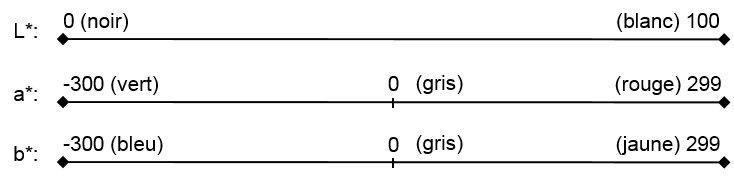
\includegraphics[scale=1]{Figures/CIELABAxes}
		\caption{Composantes de l'espace CIELAB}
		\label{fig:cielab_axes}
	\end{figure}
	
	\par La conversion de CIEXYZ vers CIELAB se fait avec les équations suivantes \citep{robertson_historical_1990}:
	\begin{equation}
		f(x)=  \begin{cases}
		x^{1/3}, & x>\left(\frac{6}{29}\right)3\\
		\frac{1}{3}\left(\frac{6}{29}\right)^2x + \frac{4}{29}, & sinon
		\end{cases}
		\label{eq:xyz_to_lab}
	\end{equation}
	
	\par Avec $X, Y, Z$ les composantes CIEXYZ de la couleur, $X_N, Y_N, Z_N$ les composantes CIEXYZ du point blanc de référence, et:
	\begin{equation}
		\begin{cases}
		L^\ast=116 \cdot f(\frac{Y}{Y_N})-16\\
		a^\ast=500 \cdot \left[f(\frac{X}{X_N})-f(\frac{Y}{Y_N})\right]\\
		b^\ast=200 \cdot \left[f(\frac{Y}{Y_N})-f(\frac{Z}{Z_N})\right]\\
		\end{cases}
	\end{equation}
	
	\par Les valeurs des coefficients des équations de L, a et b sont en fait des valeurs approchées. Les valeurs exactes sont: \[L^\ast: 117,16~et~17.16\] \[a^\ast: 509.39\] \[b^\ast: 203,75\]
	
	\par CIELAB a aussi été traduit en coordonnées cylindriques: LCh. Les composantes C et h sont les coordonnées polaires de $a^\ast$ et $b^\ast$. Ces espaces permettent de qualifier n'importe quelle couleur indépendamment de la luminosité. 
		
	\section{Observateurs standards}
	\par Tout d'abord, il convient de (re)définir les trois domaines de vision qui correspondent à des quantités d'illumination différentes (voir Fig. \ref{fig:photopic_mesopic_scotopic}) \citep{damelincourt_eclairage_2010}:
	\begin{itemize}
		\item La vision \textit{photopique} décrit la vision diurne (ou à haute luminosité). On entre dans le domaine \textit{photopique} à partir d'une illumination de $5~cd/m^2$.
		\item La vision \textit{scotopique} décrit la vision nocturne (ou à très basse luminosité). On entre dans le domaine \textit{scotopique} en dessous d'une illumination de $0.005~cd/m^2$.
		\item La vision \textit{mésopique} décrit la vision intermédiaire entre diurne et nocturne (luminosité basse). Le domaine \textit{mésopique} se situe pour une illumination entre $0.005~cd/m^2$ et $5~cd/m^2$.	
	\end{itemize}
	
	\begin{figure}[h]
		\centering
		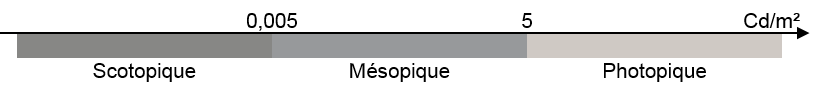
\includegraphics[scale=1]{Figures/PhotopiqueMesopiqueScotopique}
		\caption{Répartition des domaines photopique, mésopique et scotopique}
		\label{fig:photopic_mesopic_scotopic}
	\end{figure}		
	
	\par La CIE a défini le concept d' \textit{Observateur Standard} comme un profil d'efficacité lumineuse en fonction de la longueur d'onde (voir Fig. \ref{fig:standard_observer_curves}). Chaque domaine de luminosité possède son \textit{Observateur Standard}.
	
	\begin{figure}[h]
		\centering
		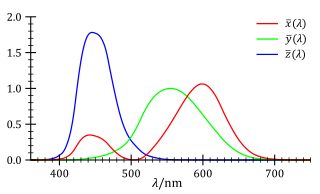
\includegraphics[scale=1]{Figures/StandardObsCurves}
		\caption{Courbes d'égalisation couleur des Observateurs Standards de la CIE}
		\label{fig:standard_observer_curves}
	\end{figure}
	
	\par Soit: $\begin{cases}
	\Phi_e(\lambda) & \textit{le flux énergétique en W (watts)}\\
	\Phi_v(\lambda) & \textit{le flux visuel en lm (lumen)}\\
	\lambda & \textit{la longueur d'onde en nm (nanomètres)}
	\end{cases}$
	
	\par En 1931, un premier \textit{Observateur Standard Photopique} pour le domaine photopique est mis au point. Il est noté $V(\lambda)$ et est valable pour un cône de vision de $2^\circ$, c'est à dire globalement la zone d'acuité de la fovéa. Cet observateur est révisé en 1964, en prenant en compte les résultats expérimentaux de plus de sujets pour calculer les coefficients. L'observateur est noté $V_{10}(\lambda)$ et couvre cette fois un cône de vision de $10^\circ$ \citep{le_grand_optique_1972, damelincourt_eclairage_2010}:
	\begin{equation}
		\begin{cases}
		\Phi_v(\lambda) = K_M \cdot V(\lambda) \cdot \Phi_e(\lambda)\\
		K_M = 683~lm.W^{-1}
		\end{cases}
		\label{eq:obs_photopic}
	\end{equation}
	
	
	\par L' \textit{Observateur Standard Scotopique} est quant à lui défini en 1951. Il est noté $V'(\lambda)$:
	\begin{equation}
		\begin{cases}
		\Phi_v(\lambda) = K'_M \cdot V'(\lambda) \cdot \Phi_e(\lambda)\\
		K'_M = 1700 lm.W^{-1}
		\end{cases}
		\label{eq:obs_scotopic}
	\end{equation}
	
	\par Enfin, il faut attendre 2010 pour voir apparaitre l'\textit{Observateur Standard Mésopique}, $V_{mes}(\lambda)$, qui n'est rien d'autre qu'une somme pondérée des deux autres observateurs en fonction de la luminance \citep{halonen_cie_2011}:
	\begin{equation}
		\begin{cases}
		\Phi_v(\lambda) = K_{mes} \cdot V_{mes}(\lambda) \cdot \Phi_e(\lambda)\\
		V_{mes}(\lambda) = (1-m) \cdot V'(\lambda) + m \cdot V(\lambda)
		K_{mes} = \frac{683}{V_{mes}[555)} lm.W^{-1}
		\end{cases}
		\label{eq:obs_mesopic}
	\end{equation}
	
	\par Les valeurs de $m$ sont fixées en dehors des bornes du domaine mésopique ($m = 1$ pour $L_{mes} \geq 5~cd/m^2$ et $m = 0$ pour $L_{mes} \leq 0.005~cd/m^2$), sinon elles sont calculées par récurrence \citep{halonen_cie_2011}:
	\begin{equation}		
	\begin{cases}
		m_0 = 0.5 & a = 0.7670\\
		m_n = a + b \cdot log_{10}(L_{mes,n}) & b = 0.3334\\
		L_{mes,n} = \frac{m_{n-1} \cdot L_{photopic} + (1-m_{n-1}) \cdot L_{scotopic} \cdot V'(\lambda_0)}{m_{n-1} + (1-m_{n-1}) \cdot V'(\lambda_0)} & \lambda_0 = 555 nm
	\end{cases}
	\label{eq:mesopic_param}
	\end{equation}
	
	\section{Illuminants}
	\par Les illuminants sont des standards de lumière déposés par la CIE (Commission Internationale de l'Eclairage) sous la forme de spectre de lumière visible (voir Fig. \ref{fig:illuminant_d65}). Chaque illuminant représente un certain type et une certaine couleur de lumière. Si l'illuminant D65 est le plus connu et le plus utilisé car il correspond à une lumière de midi en Europe occidentale, il existe plusieurs catégories.
	\begin{itemize}
	\item La classe A, déposée en 1931, représente une lumière moyenne d'une lampe à incandescence (filament en tungstène).
	\item La classe B (1931) représente la lumière directe émanant du soleil.
	\item La classe C (1931) représente la lumière du jour (après passage dans l'atmosphère).
	\end{itemize}

	\par Une deuxième vague d'illuminants a été adoptée plusieurs années après, à l'occasion de l'adoption du second observateur standard ($V_{10}(\lambda)$):
	\begin{itemize}
	\item La classe D (1964), qui se subdivise en plusieurs illuminants qui représentent les différentes phases de la lumière du jour, D65 étant midi.
	\item La classe E associée aux illuminants d'énergie égale (iso-énergie).
	\item La classe F représentant différentes lampes fluorescentes.
	\end{itemize}
	
	\begin{figure}[h]
		\centering
		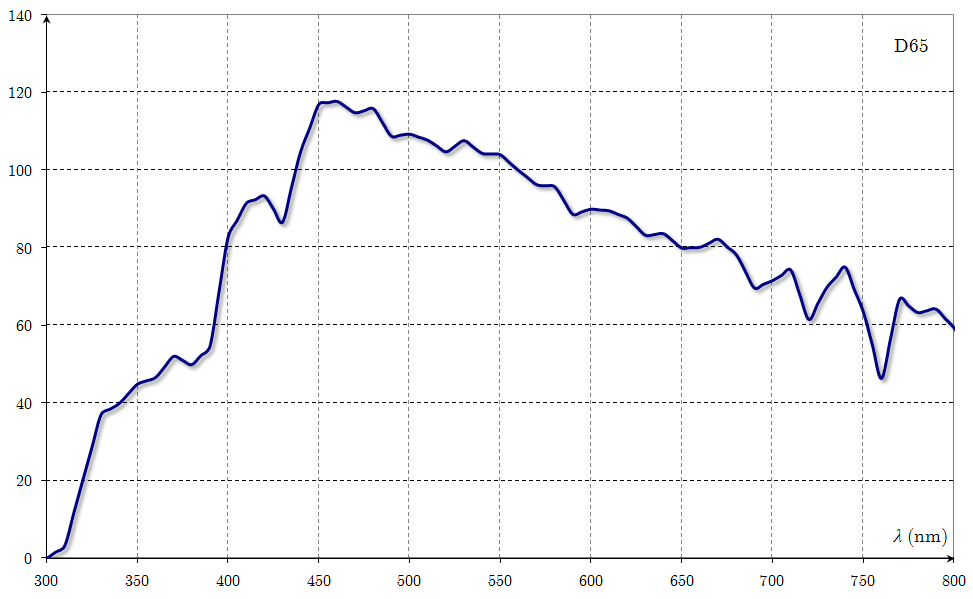
\includegraphics[scale=0.45]{Figures/IlluminantD65}
		\caption{Spectre de l'illuminant D65 (CIE)}
		\label{fig:illuminant_d65}
	\end{figure}
	
	\section{Equations de différentiations des couleurs}
	\par Une fois l'espace colorimétrique choisi, on peut dénombrer le nombre de couleurs théoriques discernables. Par exemple, dans le cas de l'espace RGB codé sur 8 bits on a 256 valeurs possibles pour chaque primaire. Lorsque l'on combine les trois primaires, on obtient un nombre théorique de 16.8 millions de couleurs. Si chacune de ces couleurs est à priori discernable, elles ne le sont pas forcément deux à deux. La CIE à donc mis en place une métrique qui indiquerait si la différence entre deux couleurs était, ou non, perceptible: $\Delta E$. Par construction, pour $\Delta E < 1$ la différence de sensation colorée n'est pas  perceptible et l'œil humain ne voit aucune différence. Empiriquement la valeur de seuil est bien plus élevée et dépend même du type de population (experte ou néophyte dans la reconnaissance de couleurs) \citep{sharma_digital_2013, vidal_color-difference_2016}.
	
	\par Il existe plusieurs équations pour calculer l'écart colorimétrique $\Delta E$, toutes ont été officialisées par la CIE en attendant des versions plus pertinentes \citep{beretta_understanding_2000, habekost_which_2013, sharma_ciede2000_2005, robertson_historical_1990}:
	\begin{itemize}
		\item CIE76
		\item CIE94
		\item CIEDE2000
		\item CMC(l,c)
	\end{itemize}
	
	\par On exprimera ici les équations dans l'espace CIELAB dans sa version originale $(L^\ast a^\ast b^\ast)$ ou dans sa version en coordonnées cylindriques $(L^\ast C h_{ab})$.
	
	\par La première équation, CIE76, est la plus simple et consiste en une simple distance euclidienne dans l'espace colorimétrique \citep{sharma_digital_2013}:
	\begin{equation}
		\Delta E_{76} = \sqrt{(\Delta L)^2 + (\Delta a)^2 + (\Delta b)^2}
		\label{eq:de_76}
	\end{equation}
	
	\par Ensuite, CIE76 a été modifiée pour s'adapter à la non linéarité de perception des couleurs \citep{beretta_understanding_2000}, elle est adoptée en 1994 et devient CIE94:
	\begin{equation}
		\Delta E^\ast_{94} = \sqrt{\left(\frac{\Delta L^\ast}{k_L \cdot S_L}\right)^2 + \left(\frac{\Delta C^\ast_{ab}}{k_C \cdot S_C}\right)^2 + \left(\frac{\Delta H^\ast_{ab}}{k_H \cdot S_H}\right)^2}
		\label{eq:de_94}
	\end{equation}
	
	\par Avec:
	$\begin{cases}
	C^\ast_{ab} = \sqrt{a^{\ast 2} + b^{\ast 2}}\\
	\Delta H^\ast_{ab} = \sqrt{\Delta E^{\ast 2}_{ab} - \Delta L^{\ast 2} - \Delta C^{\ast 2}_{ab}} = \sqrt{\Delta a^{\ast 2} + \Delta b^{\ast 2} - \Delta C^{\ast 2}_{ab}}\\
	S_C = 1 + 0.0045 \cdot C^\ast_{ab}\\
	S_H = 1 + 0.0015 \cdot C^\ast_{ab}\\
	S_L = k_L = k_C = k_H = 1
	\end{cases}$
	
	\par L'équation de 1994 résout un grand nombre de problèmes mais éprouve toujours des difficultés à décrire parfaitement le comportement de l'oeil, notamment dans le bleu. Une troisième équation est donc officialisée en 2000, CIEDE2000 \citep{schanda_colorimetry:_2007, sharma_ciede2000_2005}:
	\begin{equation}
		\Delta E^\ast_{00} = \sqrt{\left(\frac{\Delta L'}{k_L \cdot S_L}\right)^2 + \left(\frac{\Delta C'}{k_C \cdot S_C}\right)^2 + \left(\frac{\Delta H'}{k_H \cdot S_H}\right)^2 + R_T \cdot \frac{\Delta C'}{k_C \cdot S_C} \cdot \frac{\Delta H'}{k_H \cdot S_H}}
		\label{eq:de_2000}
	\end{equation}
	
	\par Le détail des coefficients de $\Delta E^\ast_{00}$ (complexe et hors de propos ici) est disponible notamment sur le site de Bruce Lindbloom\footnote{Bruce Lindbloom, \textit{Delta E (CIE 2000)}, \url{http://brucelindbloom.com/index.html?Eqn_DeltaE_CIE2000.html} (Juillet 2016)}.

	\par Enfin, si CIEDE2000 donne de très bon résultats lorsqu'il faut discriminer des couleurs de manière objective, c'est une autre équation, DECMC qui semble plus appropriée pour une discrimination subjective/perceptuelle \citep{habekost_which_2013}:
	\begin{equation}
		\Delta E(l,c) = \sqrt{\left(\frac{\Delta L}{l \cdot S_L}\right)^2 + \left(\frac{\Delta C}{c \cdot S_C}\right)^2 + \left(\frac{\Delta H}{S_H}\right)^2}
		\label{eq:de_cmc}
	\end{equation}
	
	\par Avec:
	$\begin{cases}
	(l,c) = (2,1) & \textit{pour l'acceptabilité}\\
	(l,c) = (1,1) & \textit{pour la perceptibilité}
	\end{cases}$
	
	\par De même que pour CIEDE2000, le détail des coefficients de $\Delta E(l,c)$ est disponible sur le site de Bruce Lindbloom\footnote{Bruce Lindbloom, \textit{Delta E (CMC)}, \url{http://brucelindbloom.com/index.html?Eqn_DeltaE_CMC.html} (Juillet 2016)}. On revient maintenant plus en détails sur la perception du contraste.

\chapter{Perception du contraste}
	\section{Définitions mathématiques}
	\par Tout d'abord, le dictionnaire définit le contraste comme une <<~opposition de deux choses, l'une faisant ressortir l'autre~>>\footnote{Contraste. (s.d.). Dans \textit{Dictionnaire Larousse en ligne}. Repéré à \url{http://www.larousse.fr/dictionnaires/francais/contraste/18688}}. On trouve également deux définitions plus spécifiques que sont le contraste des couleurs\footnote{Contraste des couleurs. (s.d.). Dans \textit{Dictionnaire Larousse en ligne}. Repéré à \url{http://www.larousse.fr/dictionnaires/francais/contraste/18688/locution}}: <<~effet subjectif d'une apposition quantitative de couleurs, par exemple des stimulations sensorielles juxtaposées dans l'espace (contraste simultané) ou dans le temps (contraste successif)~>> et le contraste d'une image optique\footnote{Contraste d'une image optique. (s.d.). Dans \textit{Dictionnaire Larousse en ligne}. Repéré à \url{http://www.larousse.fr/dictionnaires/francais/contraste/18688/locution}}: <<~variation relative de l'éclairement d'une image lorsqu'on se déplace à l'intérieur de cette image~>>. L'opposition se ferait ici entre le blanc et le noir pour avoir la valeur maximale du contraste.
	
	\par Ces définitions sont toutefois insuffisantes ou tout du moins inutilisables dans le monde de la vision et de l'imagerie informatique. Il faut alors théoriser plus précisément le concept de contraste et le représenter mathématiquement pour pouvoir à la fois le mesurer et le caractériser.
	Il existe pour ce faire au moins 3 méthodes analytiques, résumées ci-après:
	\begin{itemize}
		\item Le contraste de Michelson \citep{michelson_studies_1995,winkler_issues_1999,fuchs_traite_2003}.
		\item Le contraste de Weber \citep{winkler_computing_1999,winkler_issues_1999}.
		\item Le contraste de Peli \citep{peli_contrast_1990,winkler_computing_1999,winkler_issues_1999}.
	\end{itemize}

	\par Premièrement, le contraste de Michelson est défini par l'Eq. \ref{eq:contrast_michelson}, avec $L_{max}$ la valeur maximale de la luminance de l'image, et $L_{min}$ la valeur minimum. Le contraste de Michelson prend ses valeurs dans l'intervalle $\left[0;1\right]$.
	\begin{equation}
	C_{Michelson}=\frac{L_{max}-L_{min}}{L_{max}+L_{min}}
	\label{eq:contrast_michelson}
	\end{equation}

	\par Le contraste de Weber est quant à lui défini tel que dans l'Eq. \ref{eq:contrast_weber}, $\Delta L$ étant la plus petite différence de luminance visible, pour une luminance $L$ donnée. A la différence du contraste de Michelson, le contraste de Weber prend ses valeurs dans l'intervalle $\left[-1;+\infty\right[$.
	\begin{equation}
	C_{Weber}=\frac{\Delta L}{L}
	\label{eq:contrast_weber}
	\end{equation}
	
	\par Enfin, Peli a proposé un modèle de contraste pour les images complexes basé sur une analyse fréquentielle de l'image (Eq. \ref{eq:contrast_peli}). Avec $BP_{i}(x,y)$ la bande passante de l'image $i$ et $LP_{i}(x,y)$ l'énergie sous la fréquence de coupure.
	\begin{equation}
	C_{i}(x,y) = \frac{BP_{i}(x,y)}{LP_{i}(x,y)}
	\label{eq:contrast_peli}
	\end{equation}
	
	\par Malgré tout, il n'existe pas (encore) de méthode parfaite et définitive pour mesurer le contraste dans les images complexes de type image de simulateur \citep{winkler_computing_1999}. Les définitions analytiques vues à l'instant sont valables pour des images très simples et statiques.
	
	\section{Calcul de seuil}
	\subsection{Cas général}
	\par Le calcul du contraste en lui même ne suffit pas, il faut aussi savoir comment celui évolue en fonction de la luminance de l'écran: il semble assez naturel qu'à très forte luminance la capacité à distinguer un certain niveau de contraste ne soit pas la même qu'à très faible luminance. On recense ici trois modèles de comportement pour le contraste issus de la littérature:
	\begin{itemize}
		\item La fraction de Weber\footnote{Serge Bertorello, \textit{Notions d'Optique - La Vision}, \url{http://serge.bertorello.free.fr/optique/vision/vision.html} (Juillet 2016)}.
		\item Le modèle de Blackwell \citep{international_commission_on_illumination_analytic_1981}.
		\item Le modèle de Ward \citep{heckbert_contrast-based_1994}.
	\end{itemize}
	
	\par Ces modèles, notamment la fraction de Weber, ne sont souvent parfaitement valables que dans le domaine photopique (lumière du jour) et sont beaucoup plus fragiles en conditions mésopique (basse luminosité) ou scotopique (luminosité nocturne). Ils sont donc à utiliser avec prudence.

	\par Sûrement le modèle le plus connu, la fraction de Weber est dans la continuité du contraste de Weber définit précédemment. Si il s'applique notamment au contraste, ce modèle est en fait utilisable pour n'importe quel type de stimulus et est assez général. La fraction est simplement posée telle que dans Eq. \ref{eq:contrast_weber_fraction}, avec $k$ une constante, $\Delta I$ la plus petite différence d'intensité perceptible et $I$ l'intensité du stimulus. La valeur de $k$ est généralement admise à $0.02$.
	
	\begin{equation}
	\frac{\Delta I}{I} = k = 0.02
	\label{eq:contrast_weber_fraction}
	\end{equation}
	
	\par De cette fraction de Weber est issue une autre loi à propos du comportement de la rétine face à une intensité lumineuse, la loi de Weber-Fechner (Eq. \ref{eq:contrast_weber_fechner_law}). Avec $S$ la sensation perçue, $I$ l'intensité de la stimulation et $k$ une constante.
	
	\begin{equation}
	S = k \cdot log(I)
	\label{eq:contrast_weber_fechner_law}
	\end{equation}
	
	\par En 1981, la CIE a adopté un modèle établi par Blackwell et destiné au comportement du contraste en fonction de la luminance uniquement. Ce modèle donne la plus petite différence de luminance perceptible $\Delta L$ pour une luminance moyenne donnée $L_{a}$ (Eq. \ref{eq:contrast_blackwell_model}). Ici, si $\epsilon < \Delta L$, une variation de luminance $L_{a} \pm \Delta L$ est perceptible tandis que $L_{a} \pm \epsilon$ ne l'est pas car $\epsilon$ est en dessous du seuil de perception.
	
	\begin{equation}
	\Delta L(L_{a}) = 0.0594 (1.219 + L_{a}^{0.4})^{2.5}
	\label{eq:contrast_blackwell_model}
	\end{equation}
	
	\subsection{En Réalité Virtuelle}
	\par Le modèle de Ward donne un lien direct (linéaire) entre la différence minimale perceptible de luminance qui serait perçue dans le monde réel ($L_{wa}$) et son équivalent sur un dispositif d'affichage $L_{da}$ (Eq. \ref{eq:contrast_ward_model}). Le coefficient de linéarité $m$ est donné par l'Eq. \ref{eq:contrast_ward_model_m}.
	
	\begin{equation}
	\Delta L(L_{da}) = m \cdot \Delta L(L_{wa})
	\label{eq:contrast_ward_model}
	\end{equation}
	
	\begin{equation}
	m = {\left[ \frac{1.219 + (L_{da})^{0.4}}{1.219 + (L_{wa})^{0.4}} \right]}^{2.5}
	\label{eq:contrast_ward_model_m}
	\end{equation}
	
	\par Une fois ces modèles analytiques mis en place, on se rend compte assez facilement de leur lourdeur et de leur incapacité à s'adapter à des situations concrètes, notamment dans le domaine le l'informatique temps réel. Nous verrons donc dans un prochain chapitre d'autres pistes et d'autres moyens plus pratiques de quantifier le contraste.
	
	\section{Méthodes classiques de calcul sur un écran}
	\par Une première méthode classique de mesure du contraste sur un écran est la méthode dite <<~ON/OFF~>>. Elle consiste à mesurer la luminance produite par une écran lorsque celui-ci émet sa luminance maximale (c'est à dire pour un écran affiché entièrement blanc) puis la luminance minimum émise (pour écran affiché entièrement noir) et d'en faire le ratio. Si elle permet de mesurer le plus gros écart de luminance possible elle est trompeuse lorsqu'il s'agit de caractériser un écran: l'alternance noir-blanc ou blanc-noir n'est pas représentative de l'usage réel et les (futurs) utilisateurs de l'écran ne seront jamais en situation de percevoir un tel écart.
	
	\par Pour prendre en compte cette différence avec la réalité, une autre technique a été mise au point, la méthode dite ANSI (comme l'organe de régulation américain <<~American National Standards Institute~>>). Pour représenter la luminance moyenne des images habituellement affichées sur l'écran, on ne mesure plus sur des surfaces monochromes mais sur un damier noir et blanc de 4 par 4. On fait alors le ratio entre la moyenne des luminances des blancs et la moyenne des luminances des noirs. De cette manière, les zones blanches de l'écran influent sur les zones noires en augmentant leur luminance, et inversement.
	
\chapter{Perception visuelle de la profondeur}
	\par La perception de la profondeur est une des composantes fondamentales de la vision et doit faire partie des critères d'une immersion réussie. Cette perception passe par un certain nombre de principes et de paradigmes à la fois monoculaires (fonctionnement grâce à un seul œil) ou binoculaires (fonctionnement nécessairement avec les deux yeux). Les indices de profondeurs utilisés par le cerveau sont les suivants, et sont résumés et ordonnés dans la Fig. \ref{fig:indices_profondeur}:
	\begin{itemize}
	\item l' accommodation,
	\item la vergence,
	\item les disparités (horizontale et verticale),
	\item la parallaxe,
	\item les indices statiques: interposition, taille, perspective linéaire, gradient de texture, perspective aérienne, ombre, ...
	\end{itemize}
	
	\begin{figure}[h]
		\centering
		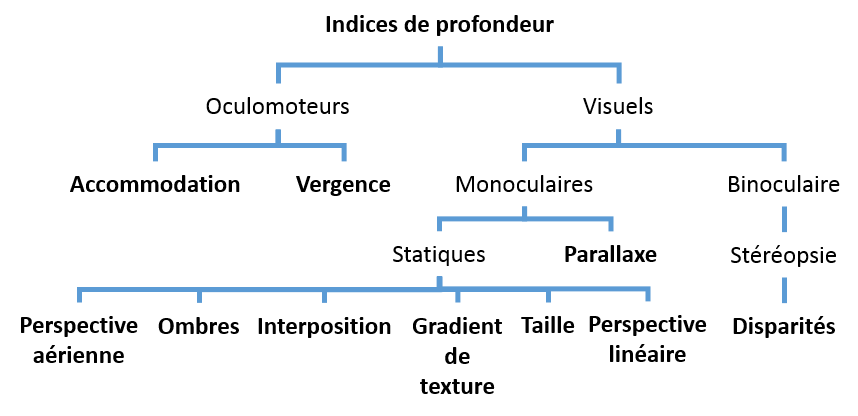
\includegraphics[scale=1]{Figures/IndicesProfondeur}
		\caption{Indices visuels de perception de la profondeur}
		\label{fig:indices_profondeur}
	\end{figure}
	
	\par Premièrement, le cerveau peut récupérer assez facilement les informations d' \textit{accommodation} et de \textit{vergence} via le principe de \textit{proprioception} évoqué plus haut. En récupérant des informations sur les muscles oculomoteurs le cerveau en déduit l'état de vergence et d' accommodation puis des informations sur la proximité de l'objet sur lequel est concentré le regard. En effet, une accommodation et une vergence à l'infini signifieront un objet éloigné et inversement. Ces indices ne sont ni les plus forts ni les plus robustes mais participent à un tout.
	
	\par La différence de disparité entre deux points permet au cerveau de comparer leurs positions respectives. Au niveau technologique cet indice est apporté par la stéréoscopie. Pour plus d'informations sur l'indice binoculaire de profondeur, on pourra se reporter à \citep{glassner_principles_1995}.
	
	\par La \textit{parallaxe}, ou parallaxe de mouvement, est un indice temporel, c'est à dire qu'il ne fonctionne pas à un instant $t$ donné mais plutôt sur une période de temps $\Delta t$. En effet, la parallaxe est l'effet sur le cerveau d'un changement de point de vue: le cerveau analyse les différences entre les images $n$ et $n+1$, et, en fonction des quantités et des vitesses de déplacement en déduit la profondeur des objets. Lorsque qu'un observateur bouge la tête en gardant le même point de fixation, tous les objets entre le point de fixation et l'observateur vont bouger avec un gradient de vitesse basé sur la distance au point de fixation (plus l'objet est éloigné, plus il va vite). Tous les points derrière le point de fixation bougeront aussi mais avec un gradient de vitesse opposé. Technologiquement, la parallaxe est assurée par la capture et l'intégration du mouvement de la tête et/ou des yeux de l'observateur dans le calcul de l'image.
	
	\par Parmi les indices statiques, l'\textit{interposition} (ou occultation) est assez simple et révélateur: si un objet masque (partiellement) un autre, alors l'objet masqué à une profondeur supérieure à l'objet masquant. Cet indice est notamment très utilisé en informatique graphique dans le pipeline de rendu\footnote{Z-buffer. Pour plus d'informations sur le pipeline de rendu: \textit{Rendering Pipeline Overview}, \url{https://www.opengl.org/wiki/Rendering_Pipeline_Overview} (Juillet 2016, en anglais).} au moment de calculer une image: tous les objets masqués sont ignorés pour le rendu de l'image (ce qui permet un gain de temps, notamment sur des scène complexes) et les objets partiellement masqués voient leur géométrie modifiée afin de ne garder que la (les) partie(s) visible(s).
	
	\par La \textit{taille} est un autre indice, basé cette fois sur notre expérience d'objets familiers dont on connait ou dont on visualise la taille. Si une voiture est vue minuscule, par expérience, on déduira que la voiture est donc loin. Cet indice ne marche qu'avec des objets que l'on connait déjà et peut être berné assez facilement (comme par exemple avec l'illusion d'optique de la chambre d'Ames).
		
	\par L'\textit{ombre} permet localement de donner des indices flagrants sur la profondeur de l'objet (voir Fig. \ref{fig:profondeur_perspectives}).
	
	\par Enfin il existe un certain nombre d'indices statiques monoculaires \citep{glassner_principles_1995, fuchs_traite_2003} que l'on peut regrouper sous la dénomination \guillemotleft~Perspective~\guillemotright . Certains de ces différents types de perspective sont illustrés Fig. \ref{fig:profondeur_perspectives}:
	\begin{itemize}
		\item Le \textit{gradient de texture} consiste à un rapprochement apparent (un écrasement des distances relatives) entre les objets de plus en plus lointains.
		\item La \textit{perspective aérienne} fonctionne pour les grandes distances uniquement: plus un objet va s'éloigner de l'observateur, plus sa couleur va perdre en intensité et fondre vers le bleu-gris (couleur de l'atmosphère), typiquement le cas des montagnes ou d'un paysage que l'on voit à l'horizon.	
		\item La \textit{perspective linéaire} est la perspective bien connue avec lignes de fuite: plus un objet s'éloigne, plus il semble rapetisser.
	\end{itemize}
	
	\par Nous avons vu le fonctionnement de la vision (modélisation du système visuel, perception de la couleur et du contraste), et son interprétation (perception de la profondeur). Néanmoins, toutes ces connaissances ne s'appliquent que dans le cas d'un sujet parfait. Nous allons maintenant présenter quelques facteurs humains (physiologiques) qui peuvent venir dégrader ou modifier la vision et ses performances.	
	
	\begin{figure}[h]
		\centering
		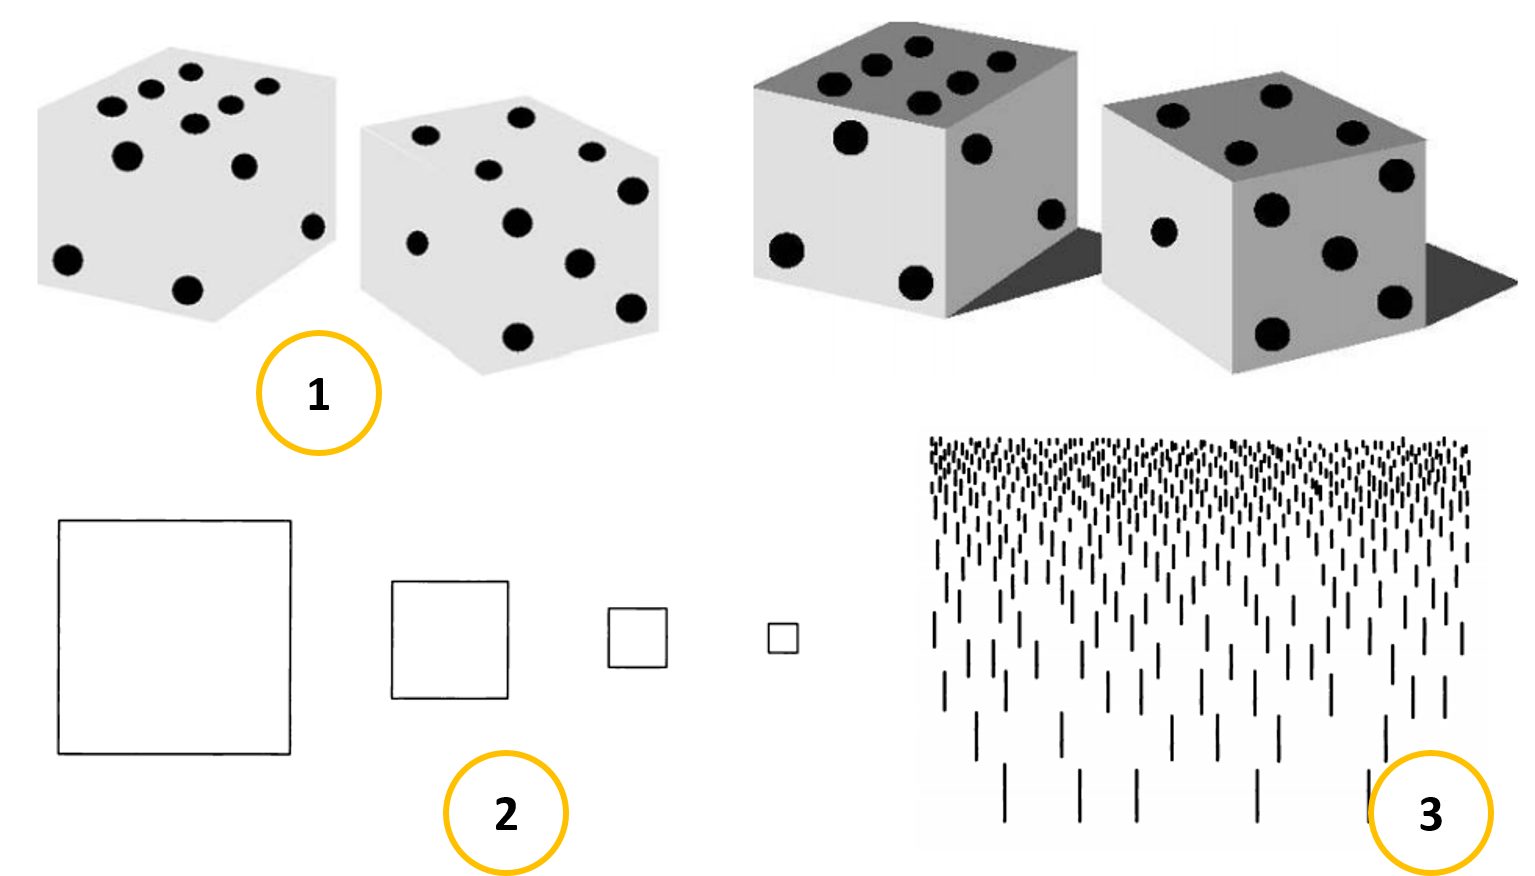
\includegraphics[scale=.25]{Figures/PerspectivesProfondeur}
		\caption{Illustration d'indices de profondeur}{Ombres (1, image tirée de \citep{anses_effets_2014}), taille et gradient de profondeur (2 et 3, images tirées de \citep{glassner_principles_1995}).}
		\label{fig:profondeur_perspectives}
	\end{figure}
	
\chapter{Influences Physiologiques}
	\par Outre les maladies ou autres défauts oculaires qui ne seront pas abordés ici, il existe un certain nombre de paramètres liés au corps humain qui influent sur la qualité de perception des images projetées par le dispositif immersif d'affichage. On trouve principalement des influences morphologiques (au niveau du visage) ou d'âge de l'observateur. On peut noter que la sensibilité au contraste est dépendante des conditions d'expérimentations évidemment, de facteurs ophtalmologiques (myopie, éblouissement rétinien, cataracte, amblyopie, dégénération de la macula avec l'âge, hyper-tension oculaire, glaucome, sécheresse oculaire) mais aussi de facteurs neurologiques (lésions cérébrales, scléroses, maladie de Parkinson et schizophrénie), ou encore de facteurs liés à la prise de médicaments \citep{pelli_measuring_2013}. Nous nous plaçons évidemment dans le cas où le sujet est sain.
		
	\section{Variations physiologiques et morphologiques}
	\par Les influences morphologiques sont très nombreuses au niveau du visage et plus ou moins faciles à caractériser et à traiter. On retrouve par exemple la distance inter-oculaire (distance entre le centre des pupilles), la profondeur des yeux, la non-horizontalité de l' alignement du centre des pupilles, le glissement des lunettes pendant l'utilisation, la position des oreilles par rapport au nez pour la position des lunettes 3D, l'écart de position entre un premier et un second port des lunettes 3D, la position du casque immersif sur le visage ... tout ce qui fait de l'observateur humain un observateur symétriquement et géométriquement imparfait.
	
	\par On développera ici le cas simple de la distance inter-oculaire. Il apparait que lorsque l'on présente les mêmes images stéréo à deux personnes différentes, la profondeur stéréoscopique des objets proches n'est pas perçue de manière égale. On prend l'exemple de l'image d'un volant de virtuel normalement paramétré pour apparaitre confondu avec le volant réel du simulateur de conduite. Certain utilisateurs verront effectivement le volant là où il est sensé être, tandis que d'autres verront l'image légèrement en avant du volant et d'autres la verront légèrement en retrait. Cet écart peut être extrêmement gênant et s'explique notamment par l'écart de distance inter-pupillaire entre les différents observateurs. Il serait cependant intéressant de comparer l'influence des différentes influences physiologiques vues précédemment afin de les hiérarchiser et éventuellement d'en négliger certaines.
	
	\par Les grandeurs ici évoquées font référence à la Fig. \ref{fig:profondeur_stereo_dio}. Pour un individu A qui a une distance interoculaire $e$, on projette sur les murs du CAVE, où dans un visio-casque, à distance $D$, un couple d'images stéréoscopiques (ici représentées par les segments vert et rouge). L'image reconstruite par le cerveau est vue à une distance $d$ par l'individu. Les images œil gauche et œil droit sont dissociées d'une distance $y$. En gardant les mêmes images, un individu B avec une distance interoculaire $e\prime$ se positionne au même endroit dans le CAVE. C'est à ce niveau là qu'intervient la différence de perception, et le second individu verra l'objet virtuel non pas à une distance $d$ mais à une distance $d\prime$ qui peut être supérieure ou inférieure à $d$.

	\begin{figure}[h]
		\centering
		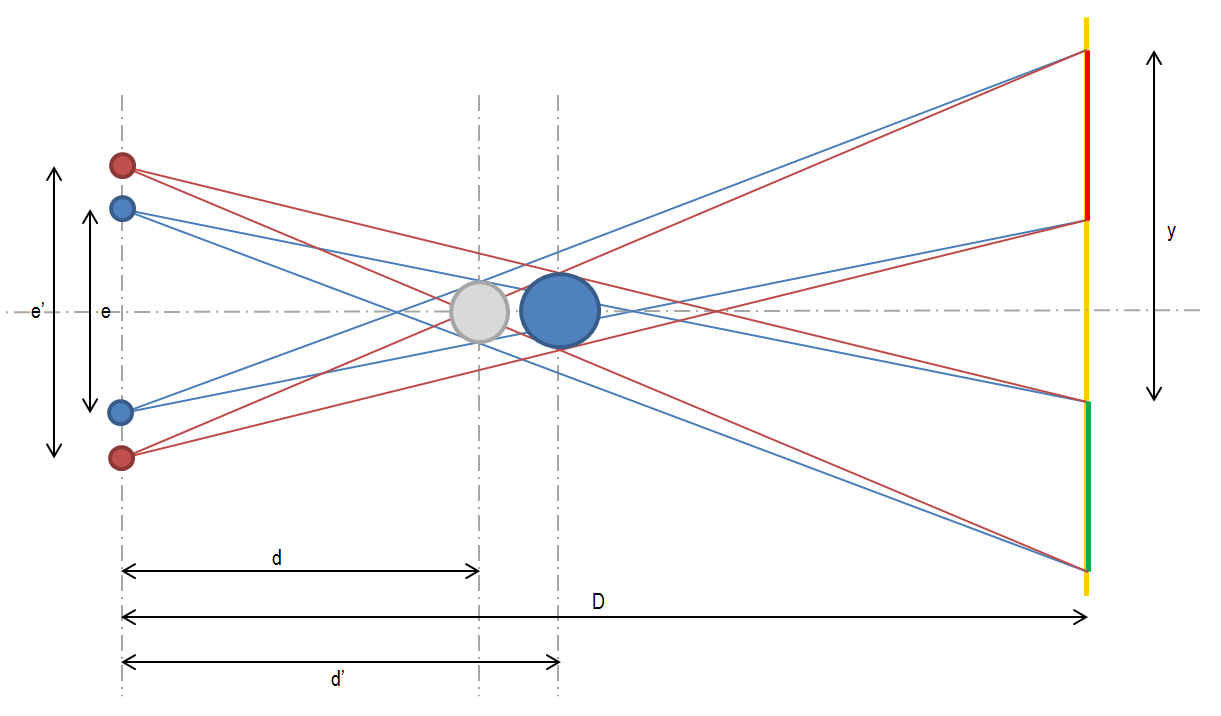
\includegraphics[scale=.5]{Figures/ProfondeurStereoDIO}
		\caption{Schématisation de la différence de profondeur stéréoscopique perçue en fonction de la distance interoculaire}
		\label{fig:profondeur_stereo_dio}
	\end{figure}

	\par En utilisant les règles élémentaires de trigonométrie (et après simplification), on trouve que la différence de distance de l'objet virtuel entre les deux individus se note de la manière suivante (Eq. \ref{eq:difference_distance_dio}):
	\begin{equation}
		\Delta d = \frac{(D - d)(e + \Delta e) - y \cdot d}{y + e + \Delta e}
		\label{eq:difference_distance_dio} 
	\end{equation}
	
	\par La Fig. \ref{fig:abaque_dio} est un abaque partiel pour une configuration donnée et pour le spectre des distances inter-oculaires possibles, de l'écart de profondeur perçue entre l'observateur A et l'observateur B pour un même jeu d'images stéréoscopiques.
	
	\par L'abaque est tracé dans la configuration spécifique avec des images projetées à la distance $D = 1.5~m$ et pour des distances de perception de l'objet en 3D de $d = 50~cm$, $75~cm$, $1~m$ et $1~m~25$. De même, on se place dans le cas général, et dans les pratiques usuelles en 3D échelle $1:1$, la distance interoculaire initiale (individu A) utilisée pour calculer le couple d'images stéréoscopiques est de 64 mm, qui est la distance interoculaire moyenne chez les hommes \citep{dodgson_variation_2004}.
	
	\par Dans le cas idéal, celui où la distance inter-oculaire n'influerait pas sur la perception de la profondeur, les images calculées pour $64~mm$ (trait orange vertical) seraient vues toujours à la même distance quelque soit la distance interoculaire (traits horizontaux en pointillés). Mais la géométrie montre bien que la réalité est toute autre (traits pleins).
	
	\par Les résultats qui émergent des courbes sont les suivants: si l'individu A perçoit l'objet virtuel à une distance de $1~m$ (courbes rouges, voir \ref{fig:abaque_dio}), un individu B avec une distance inter-oculaire de $60~mm$ (distance inter-oculaire moyenne chez les femmes \citep{dodgson_variation_2004}) verra le même objet virtuel à $980~mm$ (donc légèrement plus proche), soit avec un écart de $2~cm$ par rapport à l'observateur calculé.
	
	\begin{figure}[h]
		\centering
		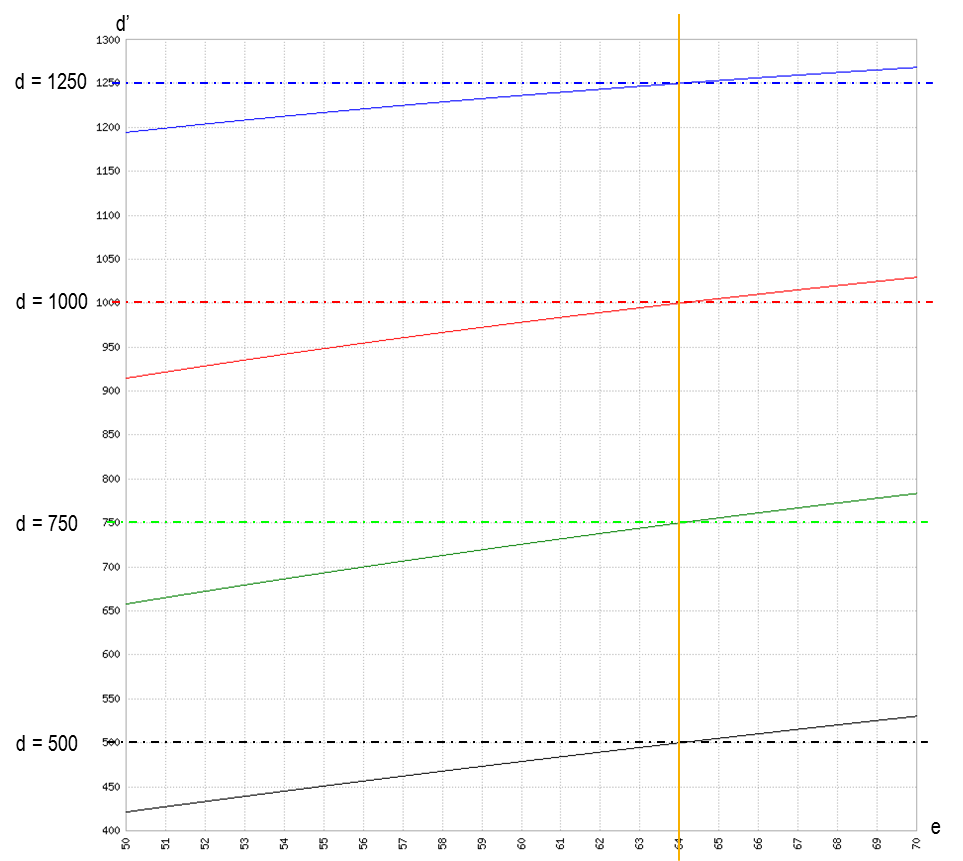
\includegraphics[scale=.8]{Figures/AbaqueDIO}
		\caption{Abaques de la nouvelle distance perçue en fonction de la distance inter-oculaire}
		\label{fig:abaque_dio}
	\end{figure}
	
	\section{Âge}
	\par L'ergonomie du système d'affichage et la physionomie du visage ne sont pas les seuls facteurs influençant la perception. Un certain nombre d'autres paramètres entrent en jeu, comme notamment le genre (homme ou femme) pour la vision des couleurs \citep{fairchild_human_2005} mais surtout, pour la quasi-totalité des grandeurs de la vision: l'âge de l'observateur.
	
	\par On peut dès lors évoquer la modification, avec l'accumulation des années, de facteurs comme le diamètre pupillaire, l'acuité visuelle ou la sensibilité au contraste \citep{owsley_contrast_1983} (voir Fig. \ref{fig:contrast_sensitivity_functions_acuity}), la réduction de la capacité à extraire des informations dans le champ de vision \citep{sekuler_effects_2000,ball_age_1988,roge_influence_2004, roge_deterioration_2009,gross_human_2008}, la qualité de l'image rétinienne \citep{artal_effects_1993}, la densité de cônes dans la fovéa \citep{kilbride_foveal_1986}, le structure de l'œil et du cristallin \citep{cook_aging_1994}.
	
	\par Par ailleurs, on recommande les vidéos de Craig Blackwell sur le thème du vieillissement de l'œil et de la vision\footnote{Craig Blackwell. 3 décembre 2014. Aging Eye 1: Vision [Vidéo en ligne]. Repéré à https://www.youtube.com/watch?v=FtcZ4an-VGo}.
	
	\begin{figure}[h]
		\centering
		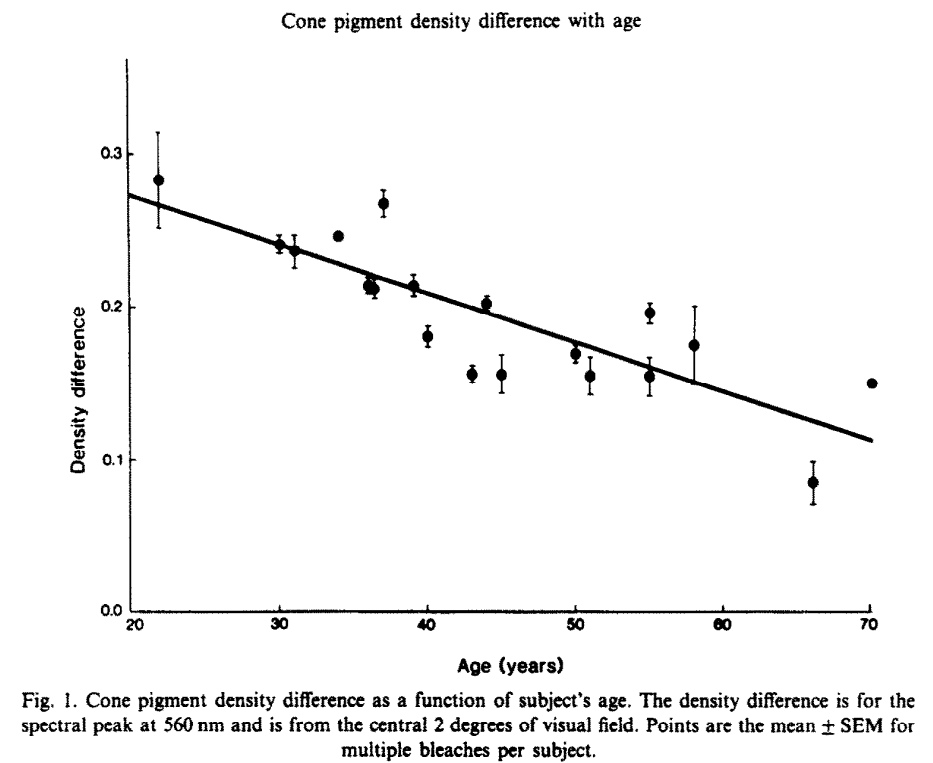
\includegraphics[scale=.5]{Figures/ConeDensityAge}
		\caption{Densité des cônes en fonction de l'âge}{Figure tirée de \citep{kilbride_foveal_1986}}
		\label{fig:densite_cones_age}
	\end{figure}